% !TEX root =../LibroTipoETSI.tex
\chapter{Transformers, Informers and Autoformers}\LABCHAP{CAP3}
\pagestyle{esitscCD}

Within the Transformer variants that have been previously exposed, three pivotal models have been selected for this thesis: the Original Transformer, the Informer, and the Autoformer. These models have been chosen due to their foundational impact and the significant advancements they introduced in the field of time series forecasting.

Firstly, analyzing the Original Transformer is crucial because it laids the groundwork for all subsequent Transformer models. Understanding its architecture and innovations provides essential insights into the core principles that underpin all Transformer-based models.

Secondly, the Informer and Autoformer models introduced relevant advancements that addressed critical challenges in time series forecasting. The Informer improved efficiency and scalability, while the Autoformer brought a novel approach to decomposing time series data. Studying these innovations helps in understanding how the field has evolved to tackle specific issues.

Furthermore, these three models have served as the basis for many other variants. By analyzing them, one can trace the evolution of ideas and techniques that have shaped the development of more specialized and advanced models. This historical perspective is essential for appreciating the progress and future directions in the field.

Finally, these models are not only theoretically significant but also practically relevant. They have been widely adopted and tested in various applications, making them valuable case studies for real-world time series forecasting challenges. By focusing on the Original Transformer, the Informer, and the Autoformer, this thesis aims to build upon their strengths and explore their applications in time series forecasting.

In this chapter, we are going to first explain what the Transformer architecture is in general. Following that, we will delve into the specifics of the time series-oriented Transformer, then the Informer, and finally the Autoformer. This structured approach will provide a clear and comprehensive understanding of each model's architecture and innovations, highlighting their contributions to the field of time series forecasting.


%%%%%%%%%%%%%%%%%%%%%%%%%%%%%%%%%%%%%%%%%%%%%%%%%%%%%%%%%%%%%%%%
\section{Transformer Architecture}

The introduction of the Transformer architecture by Vaswani et al. in 2017 marked a significant breakthrough in the field of natural language processing (NLP), fundamentally altering how machines process and understand human language. By leveraging a novel approach centered around self-attention mechanisms, the Transformer model overcame the limitations of traditional neural networks, such as recurrent neural networks (RNNs) and convolutional neural networks (CNNs), which struggled with parallelization and long-range dependencies.

The architecture's revolutionary nature lies in its ability to eschew sequential data processing, allowing for the parallelization of operations and significantly improving computational efficiency. Composed of an encoder-decoder structure built from layers of self-attention and feed-forward neural networks, the Transformer excels at handling long-range dependencies within sequences. This makes it exceptionally well-suited for complex NLP tasks such as machine translation, text summarization, and question answering, where understanding context and maintaining coherence across lengthy texts are paramount.

Next, we will delve into the intricacies of the Transformer's encoder-decoder architecture, detailing the role of each component and how they work together to enable high-performance language processing. We will also explore the self-attention mechanism, which lies at the heart of the Transformer's success, allowing it to dynamically weigh the importance of different elements in an input sequence and capture intricate dependencies within the data. This section will further highlight the advantages of multi-head attention and explain how these innovations contribute to the model's robustness and versatility.


\begin{figure}[htbp]
    \centering
    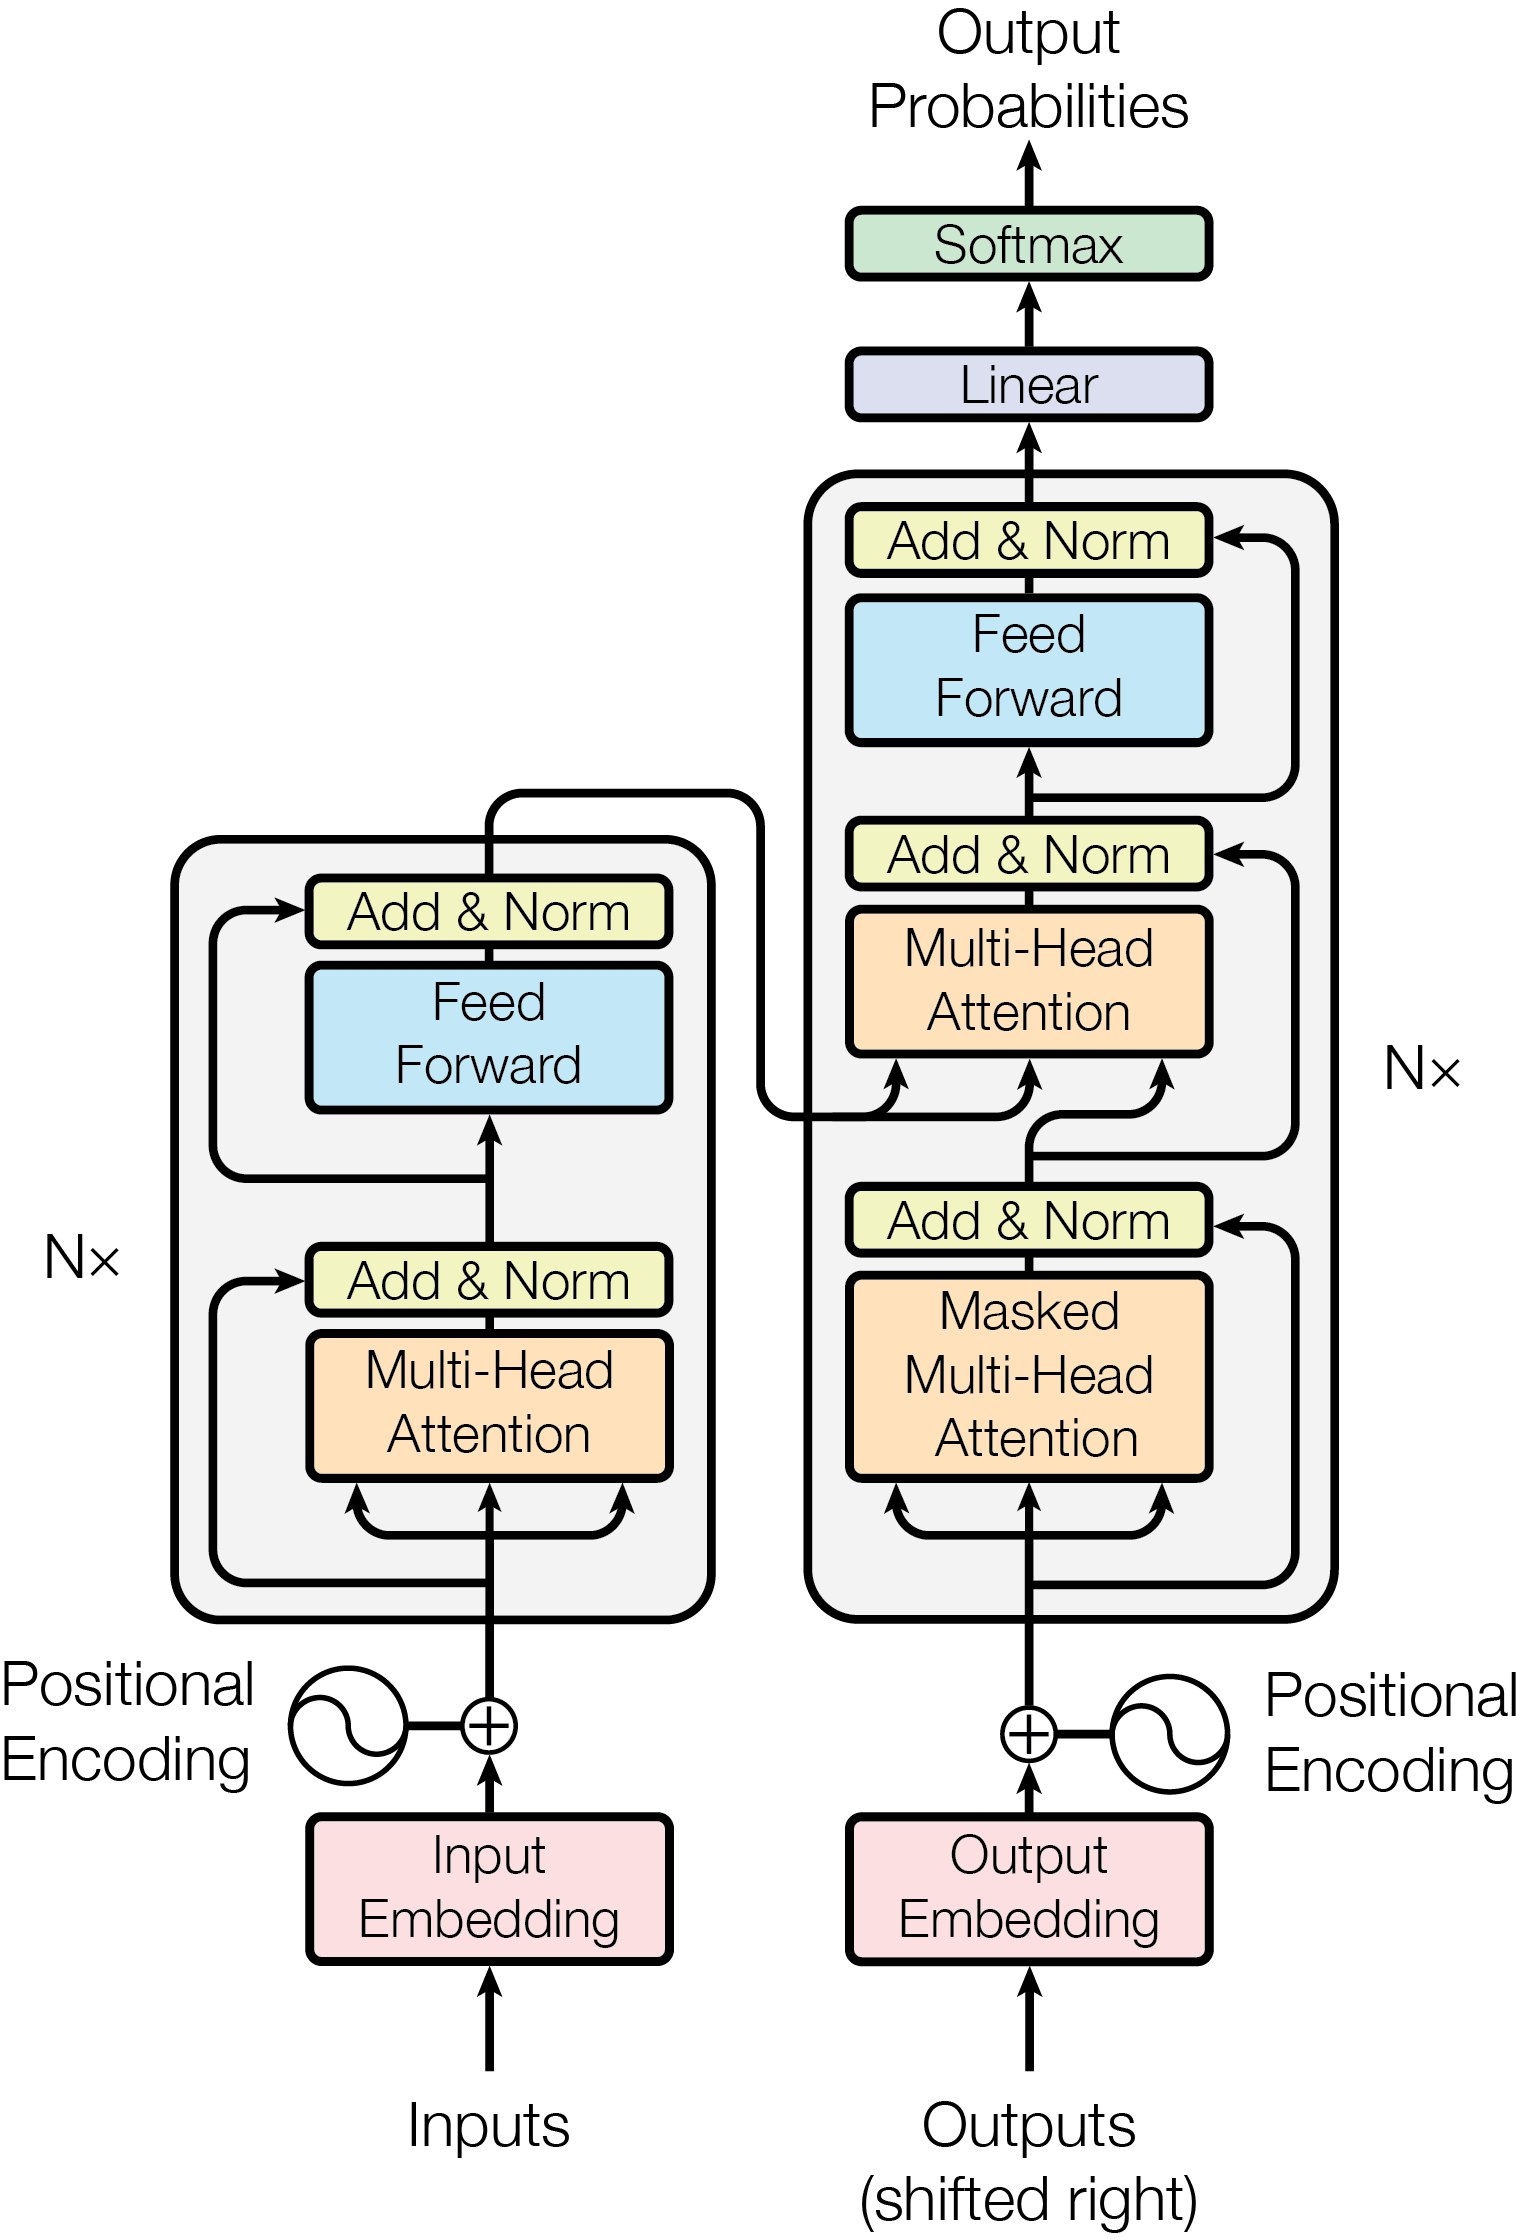
\includegraphics[width=6 cm]{3_ChapterTranformerVariants/figuras/Transformer_architecture.png}
    \caption{The Transformer - model architecture, from \textit{"Attention Is All You Need"} (Vaswani, et al., 2017)~\cite{vaswani2023attention}}
    \LABFIG{FIG}
    \end{figure}

\subsubsection{Encoder-Decoder Structure}

\noindent\textbf{Encoder}

\noindent Each encoder layer in the Transformer model is composed of two primary sub-layers. The first sub-layer is the multi-head self-attention mechanism. This mechanism allows the model to focus on different parts of the input sequence simultaneously, capturing various aspects of the input data. By using multiple attention heads, the model can learn to attend to different positions in the sequence, which helps in understanding the context and relationships between different elements in a sequence more effectively.

The second sub-layer is the fully connected feed-forward network. This network is applied to each position independently and identically, consisting of two linear transformations with a ReLU activation in between. This sub-layer helps in further processing the information extracted by the self-attention mechanism, adding non-linearity and enabling the model to learn more complex patterns.

Both sub-layers are followed by layer normalization and residual connections. Layer normalization helps in stabilizing the training process by normalizing the inputs to each sub-layer, while residual connections allow the model to retain information from previous layers, facilitating better gradient flow and improving the overall training efficiency.
\vspace{10pt}

\noindent\textbf{Decoder}

\noindent The decoder in the Transformer model also consists of multiple layers, each containing three main sub-layers. The first sub-layer is the masked multi-head self-attention mechanism. Unlike the encoder's self-attention, this mechanism is masked to prevent the decoder from attending to future positions in the sequence, ensuring that the prediction for a particular position only depends on the known outputs up to that position.

The second sub-layer is the encoder-decoder attention mechanism. This mechanism allows the decoder to focus on relevant parts of the input sequence by attending to the encoder's output. It helps the decoder to incorporate information from the entire input sequence, which is crucial for generating accurate and contextually appropriate outputs.

The third sub-layer is the same fully connected feed-forward network used in the encoder. This sub-layer further processes the combined information from the self-attention and encoder-decoder attention mechanisms.

Similar to the encoder, each of these sub-layers in the decoder is followed by layer normalization and residual connections. These components ensure stable training and efficient information flow throughout the network.
\vspace{10pt}

\subsubsection{Self-Attention Mechanism}
At the core of the Transformer architecture is the self-attention mechanism, which enables the model to weigh the importance of different elements in an input sequence dynamically. The self-attention mechanism computes a set of attention scores for each element in the sequence, determining how much focus each element should have on every element in the sequence.
\vspace{10pt}

\noindent\textbf{Scaled Dot-Product Attention}

\noindent The self-attention mechanism operates through a process called scaled dot-product attention, which can be broken down into several key steps:

\begin{enumerate}
    \item \textbf{Calculate Query (Q), Key (K), and Value (V) Vectors}: For each element in the input sequence, the model generates three vectors: a query vector (Q), a key vector (K), and a value vector (V). These vectors are derived from the element embeddings using learned linear transformations.
    \item \textbf{Compute Attention Scores}: The attention score for each element pair is computed by taking the dot product of the query vector of the current element with the key vector of another element. This measures the relevance of one element to another.
    \item \textbf{Scale the Attention Scores}: To prevent the dot product values from becoming too large and destabilizing the learning process, the attention scores are scaled by dividing by the square root of the dimensionality of the key vectors ($\sqrt{d_k}$).
    \item \textbf{Apply Softmax Function}: The scaled attention scores are then passed through a softmax function to convert them into probabilities, ensuring that the scores for each element sum to 1. These probabilities are known as attention weights.
    \item \textbf{Weighted Sum of Value Vectors}: The final attention output for each element is obtained by taking a weighted sum of the value vectors, using the attention weights as coefficients.
\end{enumerate}

The entire process is summarized by the following formula:

\begin{equation}
\text{Attention}(Q, K, V) = \text{softmax}\left(\frac{QK^T}{\sqrt{d_k}}\right)V \text{ .}
\end{equation}

\begin{figure}[htbp]
    \centering
    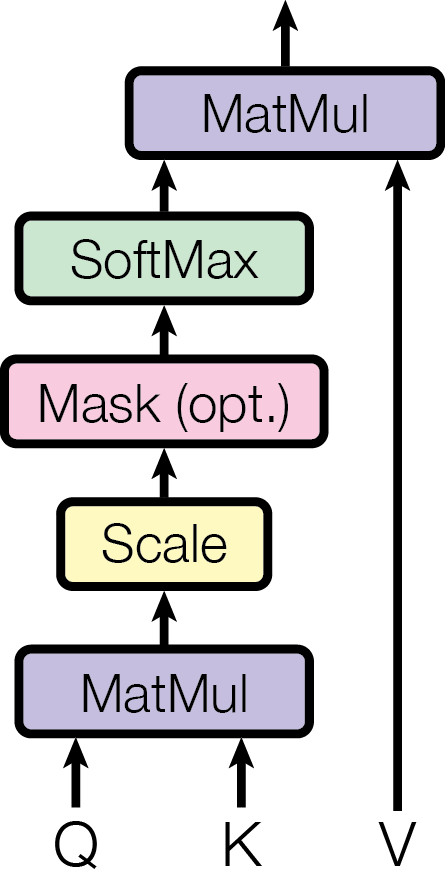
\includegraphics[width=3 cm]{3_ChapterTranformerVariants/figuras/ScaledDotProductAttention.png}
    \caption{Scaled Dot-Product Attention, from \textit{"Attention Is All You Need"} (Vaswani, et al., 2017)~\cite{vaswani2023attention}}
    \LABFIG{FIG}
    \end{figure}

\noindent\textbf{Multi-Head Attention}

\noindent Instead of performing a single attention function, the Transformer employs multiple attention heads. Each head performs its own attention operation in parallel, allowing the model to capture different aspects of relationships between different elements in sequence. The outputs of all heads are then concatenated and linearly transformed to produce the final attention output.

\begin{equation}
\text{MultiHead}(Q,K,V) = \text{Concat}(\text{head}_1, \ldots, \text{head}_h) W^O \text{ ,}
\end{equation}where each head is defined as:

\begin{equation}
\text{head}_i = \text{Attention}(QW_i^Q, KW_i^K, VW_i^V) \text{ .}
\end{equation}

\begin{figure}[htbp]
    \centering
    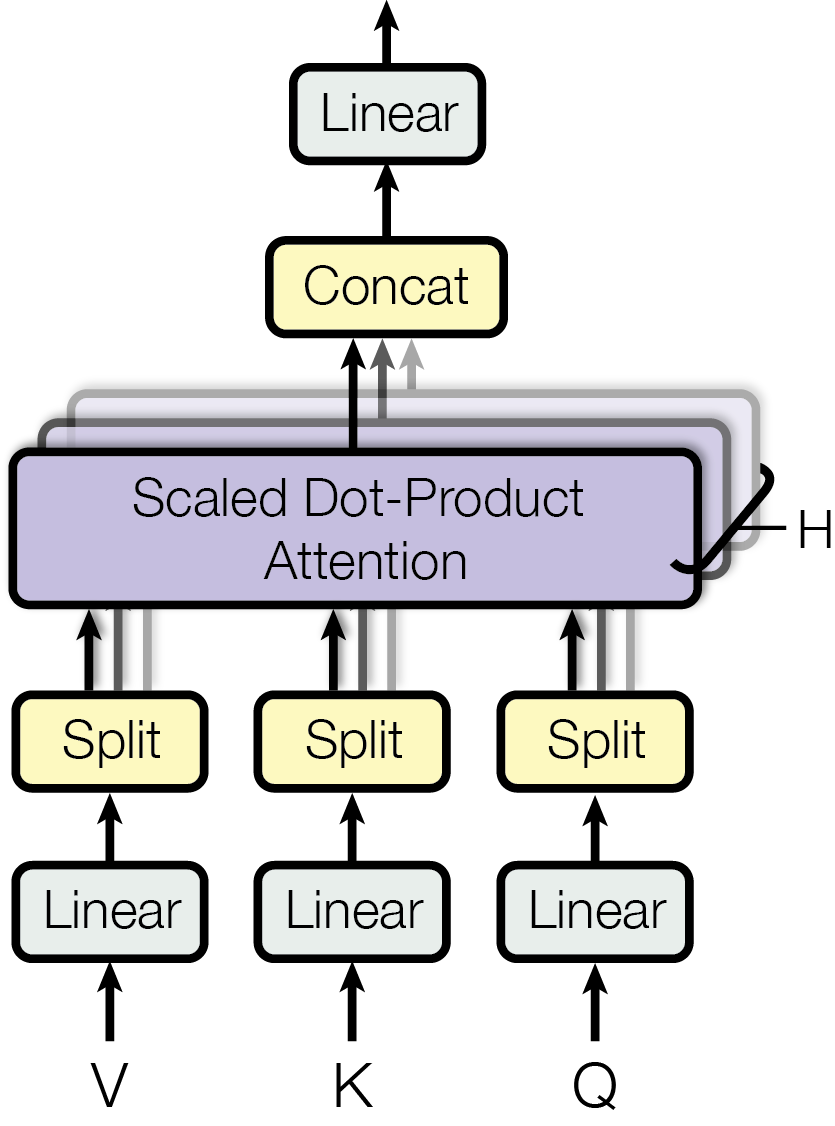
\includegraphics[width=5cm]{3_ChapterTranformerVariants/figuras/MultiHeadAttention.png}
    \caption{Multi-Head Attention, from \textit{"Attention Is All You Need"} (Vaswani, et al., 2017)~\cite{vaswani2023attention}}
    \LABFIG{FIG}
    \end{figure}

%%%%%%%%%%%%%%%%%%%%%%%%%%%%%%%%%%%%%%%%%%%%%%%%%%%%%%%%%%%%%%%%
\section{Time Series Transformer}

Previously, we explored the Transformer architecture. Now, we turn our focus to the Time Series Transformer, designed specifically for time series forecasting. As well as the original Transformer, this model is built around two main components: the Encoder and the Decoder. The Encoder processes past time series values, capturing essential patterns and dependencies. Meanwhile, the Decoder uses this encoded information to predict future values, integrating temporal features to enhance prediction accuracy.

Time series forecasting involves predicting future values based on historical data. The Time Series Transformer tackles this through embeddings, which convert categorical data into continuous vectors, capturing temporal dependencies effectively. These embeddings include channel projection and timestamp embeddings, which help the model understand both local and global temporal dynamics.

Training the model involves a method called teacher-forcing, where the model learns correct sequence patterns by using actual previous values during training. Additionally, the Time Series Transformer employs probabilistic forecasting to quantify uncertainty in predictions, which is crucial for real-world decision-making.

\subsection{Time Series Forecasting (TSF) Problem Formulation}
Time series forecasting (TSF) involves predicting future values based on previously observed data. For a time series containing \(C\) variates, the historical data can be represented as:

\begin{equation}
X = \{X^t_1, \ldots, X^t_C\}_{t=1}^L \text{ ,}
\end{equation}where \(L\) is the look-back window size and \(X^t_i\) is the value of the \(i\)-th variate at the \(t\)-th time step. The goal of TSF is to predict the future values:

\begin{equation}
\hat{X} = \{\hat{X}^t_1, \ldots, \hat{X}^t_C\}_{t=L+1}^{L+T}
\end{equation}for the next \(T\) time steps.

When \(T > 1\), there are two main approaches to multi-step forecasting:
\begin{itemize}
    \item \textbf{Iterated Multi-Step (IMS) Forecasting:} This approach learns a single-step forecaster and iteratively applies it to obtain multi-step predictions. While IMS predictions tend to have smaller variance due to the autoregressive estimation procedure, they are prone to error accumulation effects. Therefore, IMS forecasting is preferable when there is a highly accurate single-step forecaster and \(T\) is relatively small.
    \begin{figure}[htbp]
        \centering
        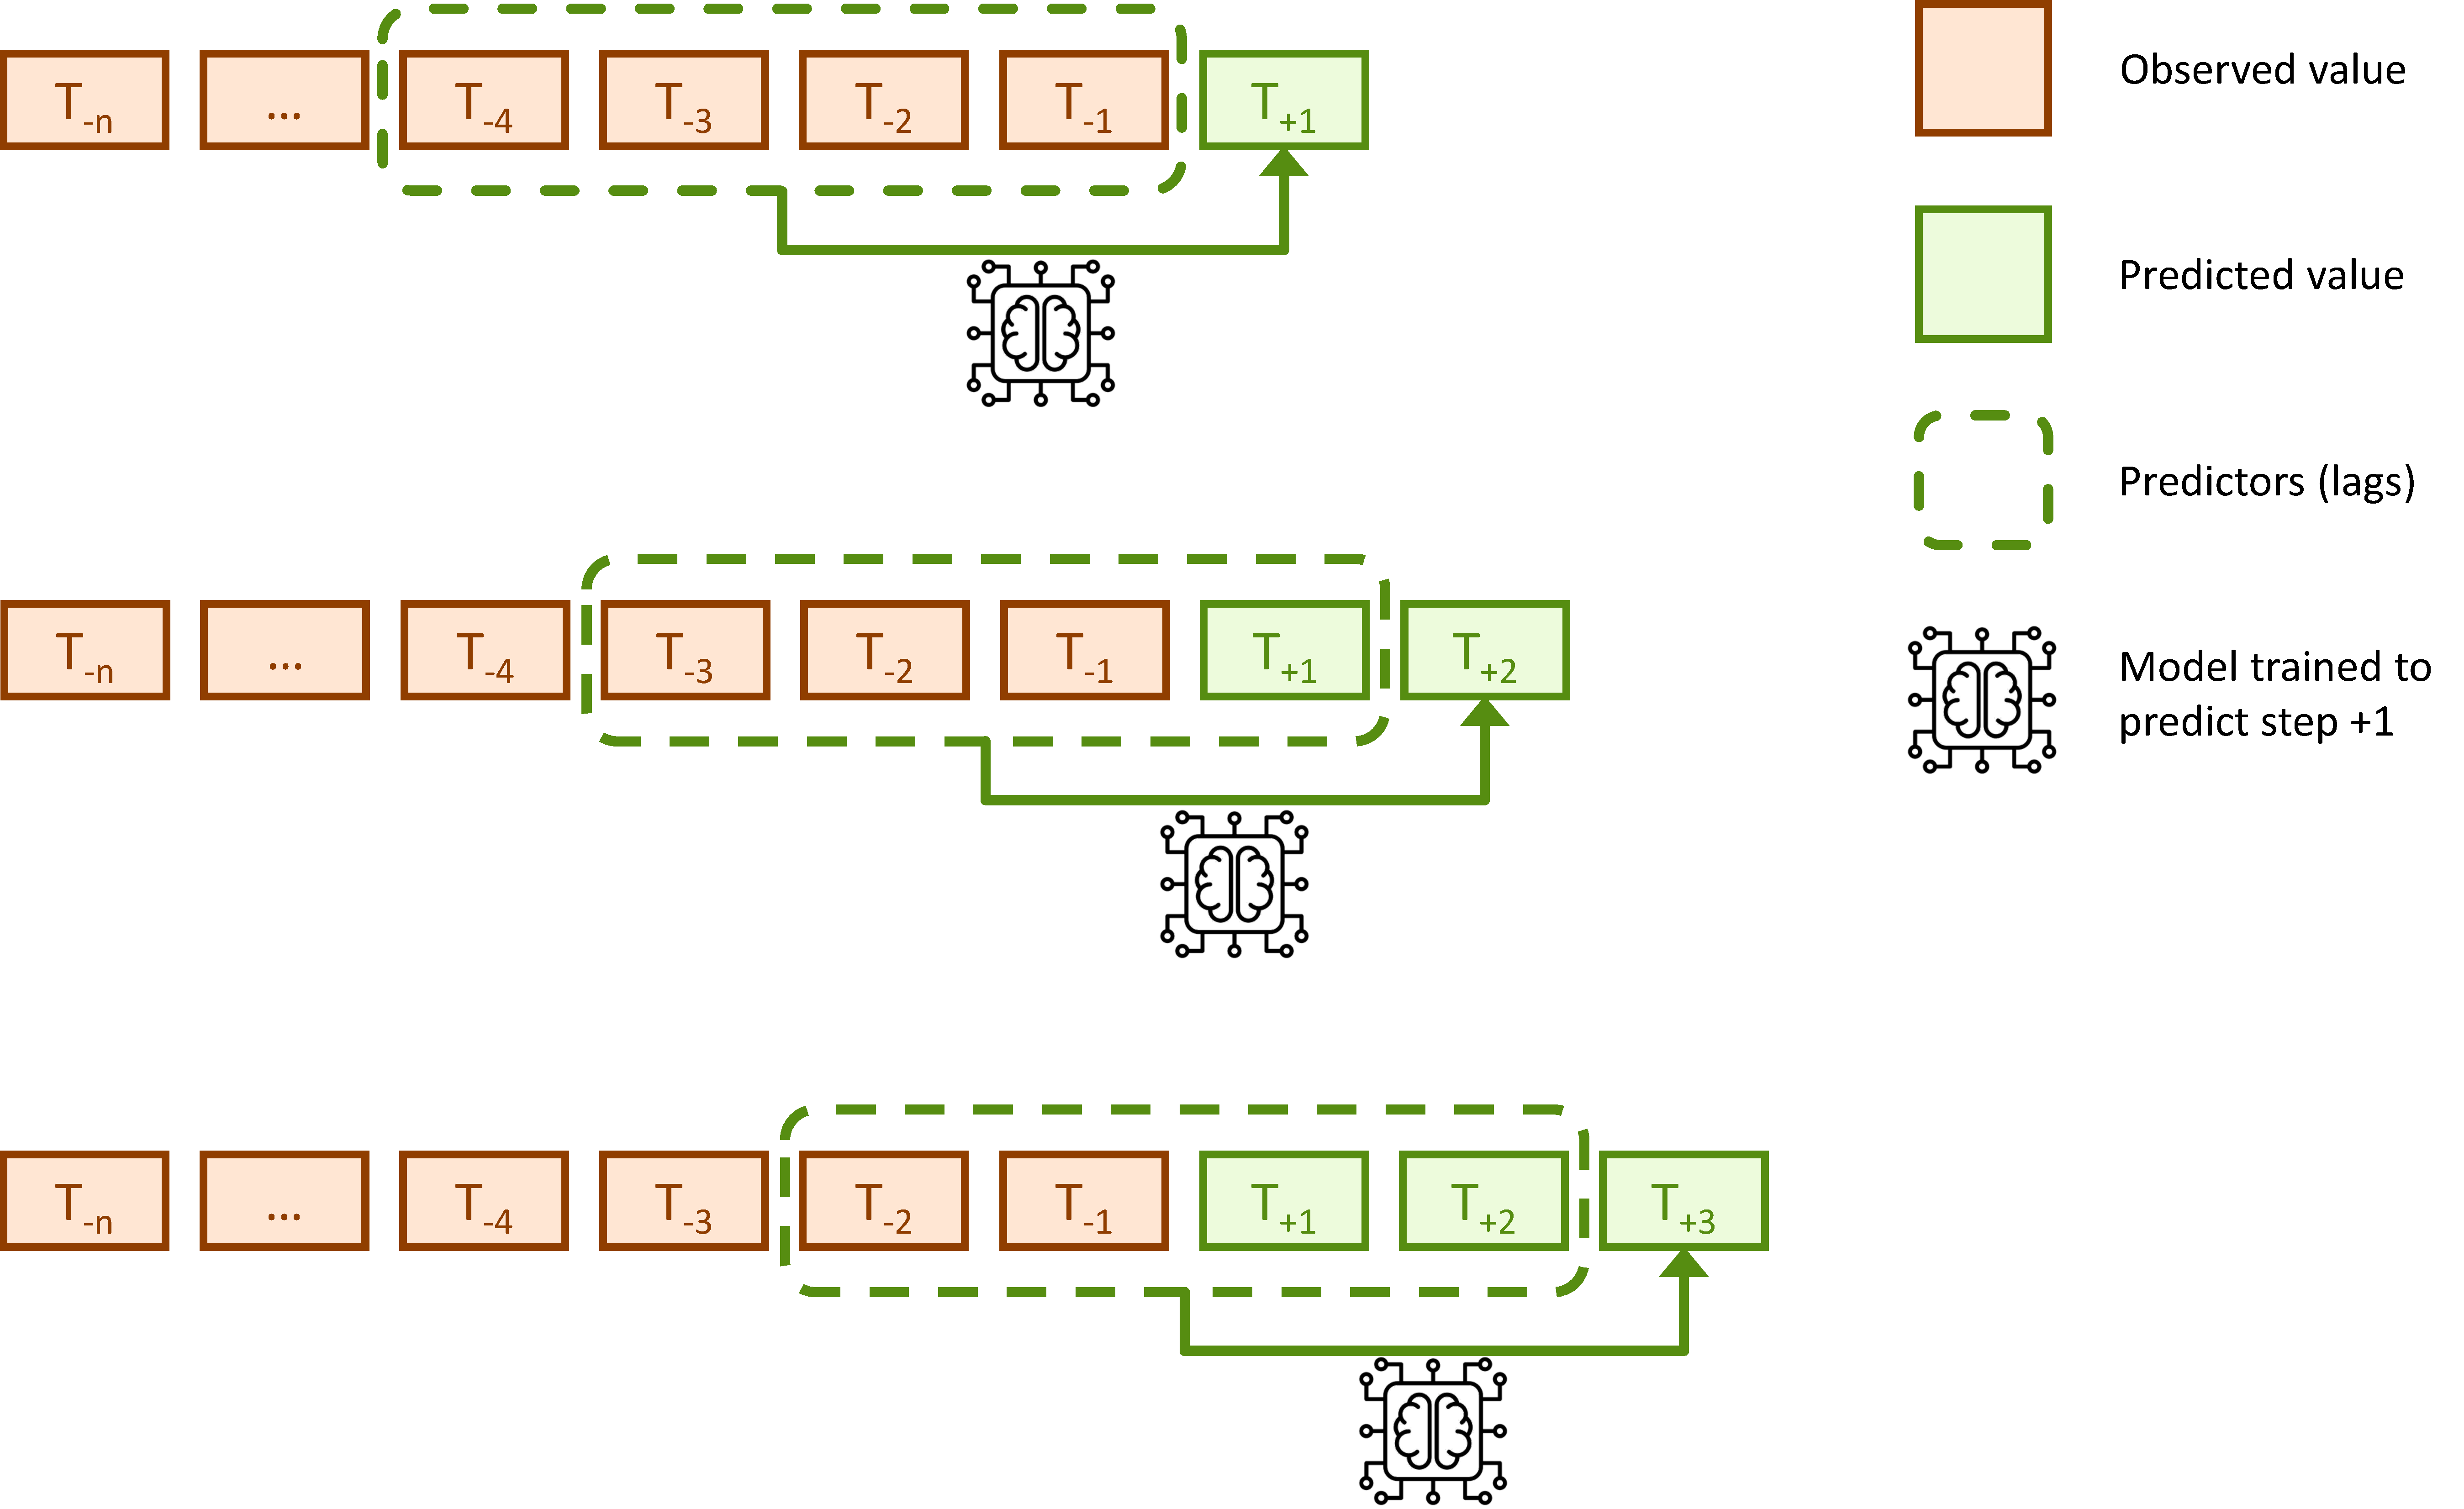
\includegraphics[width=13cm]{3_ChapterTranformerVariants/figuras/IMS.pdf}
        \caption{Illustration of Iterated Multi-Step (IMS) Forecasting}
        \LABFIG{FIG}
        \end{figure}
    
    \item \textbf{Direct Multi-Step (DMS) Forecasting:} This approach directly optimizes the multi-step forecasting objective at once. DMS forecasting generates more accurate predictions when it is challenging to obtain an unbiased single-step forecasting model or when \(T\) is large.
    \begin{figure}[htbp]
        \centering
        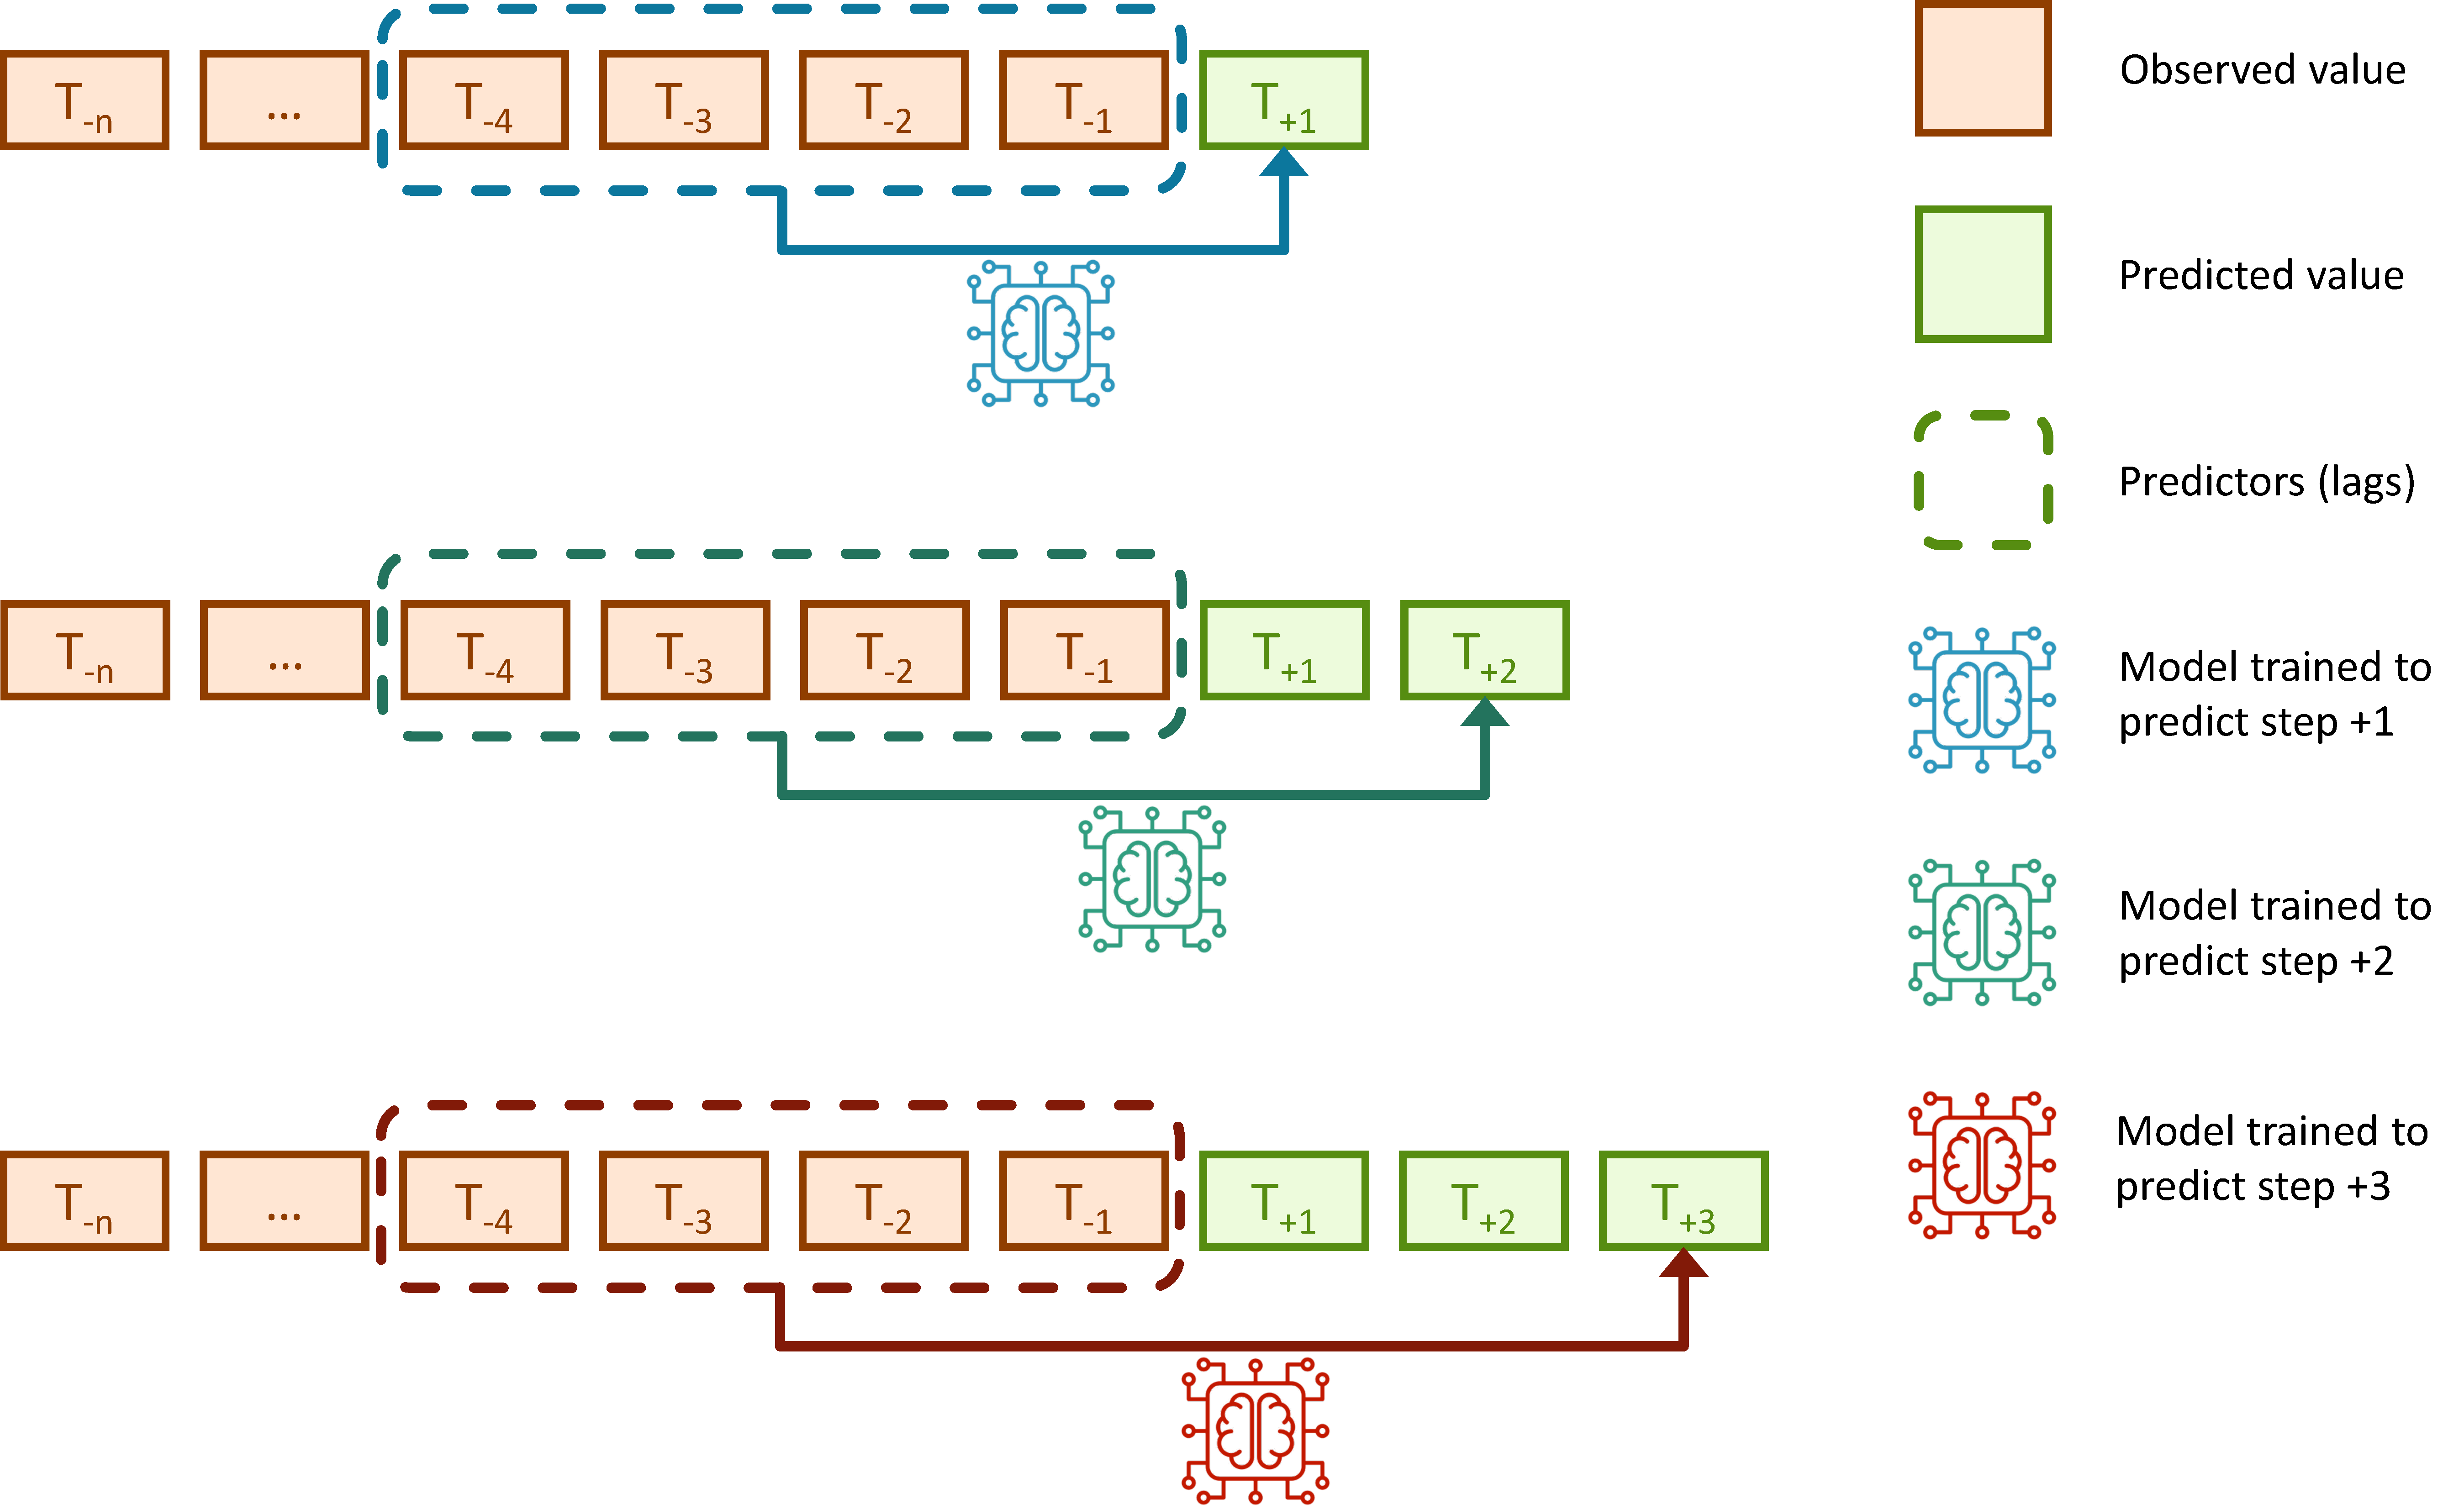
\includegraphics[width=13cm]{3_ChapterTranformerVariants/figuras/DMS.pdf}
        \caption{Illustration of Direct Multi-Step (DMS) Forecasting}
        \LABFIG{FIG}
        \end{figure}
    
\end{itemize}

\subsection{Embedding}
Embeddings are a crucial component in the field of machine learning and natural language processing. They are used to convert categorical data into continuous vector representations, which can then be fed into machine learning models. In the context of time series forecasting, embeddings help in capturing the temporal dependencies and patterns within the data, enabling the model to make accurate predictions.

To adapt the Transformer architecture for time series forecasting, the embedding process involves several key components: channel projection, fixed position, local timestamp, and global timestamp. Each of these components plays a vital role in ensuring that the model effectively captures the temporal dynamics of the data.

\subsubsection{Channel Projection}
Channel projection is the process of transforming the input time series data into a higher-dimensional space. This is done to capture the complex relationships between different channels (or features) of the time series data. By projecting the data into a higher-dimensional space, the model can better understand the interactions between different channels and make more accurate predictions.
\begin{figure}[htbp]
    \centering
    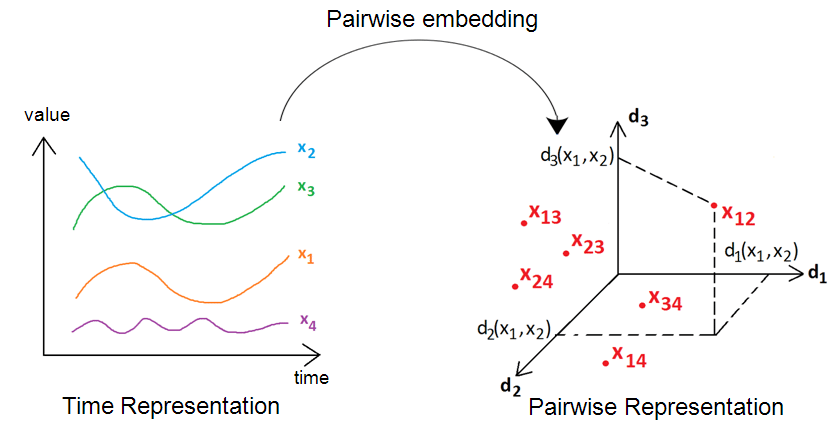
\includegraphics[width=13cm]{3_ChapterTranformerVariants/figuras/ChannelProjection.png}
    \caption{Example of embedding of time series xi from the temporal space (left) into the pairwise space (right). In this example, a pair of time series (x1, x2) is projected into the pairwise space as a vector x12 described by p = 3 basic metrics: x12 = [d1(x1, x2), d2(x1, x2), d3(x1, x2)] T, from \textit{"Multiple Metric Learning for large margin kNN Classification of time series"}~\cite{inproceedings}}
    \LABFIG{FIG}
    \end{figure}

\subsubsection{Fixed Position Embedding}
As we explained before, fixed position embedding is used to encode the positional information of the time series data. In the Transformer architecture, positional encodings are added to the input embeddings to provide the model with information about the order of the data points. This is crucial for time series forecasting, as the temporal order of the data points is essential for making accurate predictions. Fixed position embeddings are typically generated using sinusoidal functions, which provide a unique encoding for each position in the sequence.

\subsubsection{Local Timestamp Embedding}
Local timestamp embedding captures the local temporal information within the time series data. This includes information such as the time of day, day of the week, or any other relevant local temporal features. By incorporating local timestamp embeddings, the model can better understand the short-term patterns and trends within the data, leading to more accurate forecasts.

For example, consider a data point recorded at 3 PM on a Wednesday. The local timestamp embedding would capture the hour of the day (15), the day of the week (3 for Wednesday), and the day of the month (15).

\subsubsection{Global Timestamp Embedding}
Global timestamp embedding captures the global temporal information across the entire time series. This includes long-term trends and seasonal patterns that may not be immediately apparent from the local temporal information. By incorporating global timestamp embeddings, the model can better understand the overall temporal dynamics of the data, leading to more accurate long-term forecasts.

For example, imagine a data point recorded in July 2024. The global timestamp embedding would include the month of the year (7 for July), the quarter of the year (3 for July to September), and the year (2024).

\begin{figure}[htbp]
    \centering
    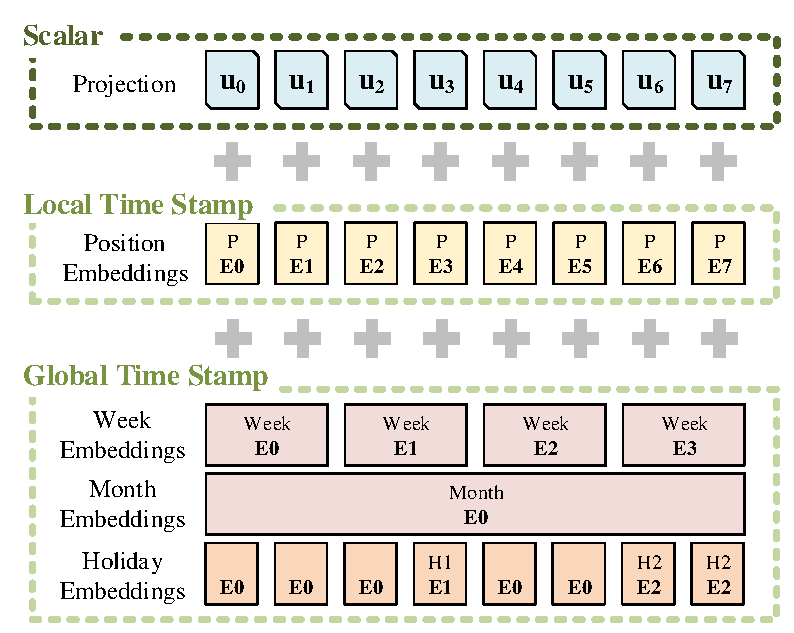
\includegraphics[width=10cm]{3_ChapterTranformerVariants/figuras/Embbeding.pdf}
    \caption{The input representation of a Time Series Transformer, from Informer (Zhou, et al., 2019)~\cite{zhou2021informerefficienttransformerlong}}
    \LABFIG{FIG}
    \end{figure}



\subsection{Encoder}
The Encoder’s role is to process a sequence of past time series values, known as \textit{past\_values}. It effectively captures the temporal patterns and dependencies within these values. In addition to the raw \textit{past\_values}, the Encoder takes the data from the embedding, which includes local timestamps and other relevant temporal features, to provide the model with more temporal context.

\subsection{Decoder}
The Decoder’s role is to predict future time series values, known as \textit{future\_values}, based on the encoded information from \textit{past\_values}. The Decoder generates a sequence of predictions for the desired forecast horizon. Like the Encoder, the Decoder can incorporate future time features to provide temporal context for the predictions. These features are analogous to the past time features.

\subsection{Training Methodology}
Training a Time Series Transformer involves a process called \textit{teacher-forcing}. This method is crucial for effectively training sequence-to-sequence models, such as those used in time series forecasting.

Teacher-forcing is a technique where the model is trained to predict the next value in a sequence by using the actual previous value rather than the model's own previous prediction. This helps the model learn the correct sequence patterns more efficiently and reduces the accumulation of errors during training.

Here's a step-by-step breakdown of how we train the Time Series Transformer:
\begin{enumerate}
    \item \textbf{Preparing the Training Data:}
    \begin{itemize}
        \item We start with pairs of \textit{past\_values} and \textit{future\_values}.
        \item \textit{past\_values} represent the known historical data up to the current time step.
        \item \textit{future\_values} represent the target values we aim to predict.
    \end{itemize}
    \item \textbf{Shifting Future Values:}
    \begin{itemize}
        \item The \textit{future\_values} sequence is shifted one position to the right.
        \item This creates a new sequence where each time step corresponds to the next time step in the original \textit{future\_values}.
    \end{itemize}
    \item \textbf{Initial Input for the Decoder:}
    \begin{itemize}
        \item The last value of \textit{past\_values} is used as the initial input for the Decoder.
        \item This value acts as the starting point for generating the first prediction in the \textit{future\_values} sequence.
    \end{itemize}
    \item \textbf{Training with Teacher-Forcing:}
    \begin{itemize}
        \item During training, the model uses the actual previous value from the \textit{future\_values} sequence as the input for the next time step.
        \item This ensures that the model is conditioned on the correct context at each step, helping it learn the dependencies more accurately.
    \end{itemize}
    \item \textbf{Loss Calculation and Backpropagation:}
    \begin{itemize}
        \item The model's predictions are compared to the actual \textit{future\_values} to calculate the loss.
        \item The loss is then backpropagated through the model to update the weights and improve the predictions.
    \end{itemize}
\end{enumerate}

The use of teacher-forcing in training Time Series Transformers is essential for achieving accurate and stable predictions. By providing the model with the correct context at each step, we ensure that it learns the correct sequence patterns and dependencies, leading to better performance in time series forecasting tasks.


\subsection{Probabilistic Forecasting}
Unlike classical point forecasting methods that output a single value per time step, the Time Series Transformer is designed for probabilistic forecasting. This approach models a distribution from which predictions can be sampled, providing a measure of uncertainty in the forecasts. This is particularly useful in real-world decision-making processes where understanding the range of possible outcomes is crucial.

Deep learning models, including Transformers, excel in this context by learning from multiple related time series and modeling data uncertainty effectively. Probabilistic forecasting can be implemented by learning future parameters of a parametric distribution or using techniques like conformal prediction adapted for time series.

According to the paper \textit{"Use and Communication of Probabilistic Forecasts"} (Adrian E. Raftery)~\cite{raftery2014usecommunicationprobabilisticforecasts}, probabilistic forecasts are becoming increasingly available and are essential for various types of users, including general assessors, change assessors, risk avoiders, and decision theorists. These forecasts provide valuable insights by quantifying the uncertainty and offering a range of possible outcomes, which can be summarized using probabilities of adverse events and percentiles of the predictive distribution. Effective communication of probabilistic forecasts involves interacting with users to understand their goals and minimizing cognitive load by presenting the information in a clear and concise manner. This ensures that the forecasts are not only accurate but also trusted and actionable in practical applications.

\begin{figure}[htbp]
    \centering
    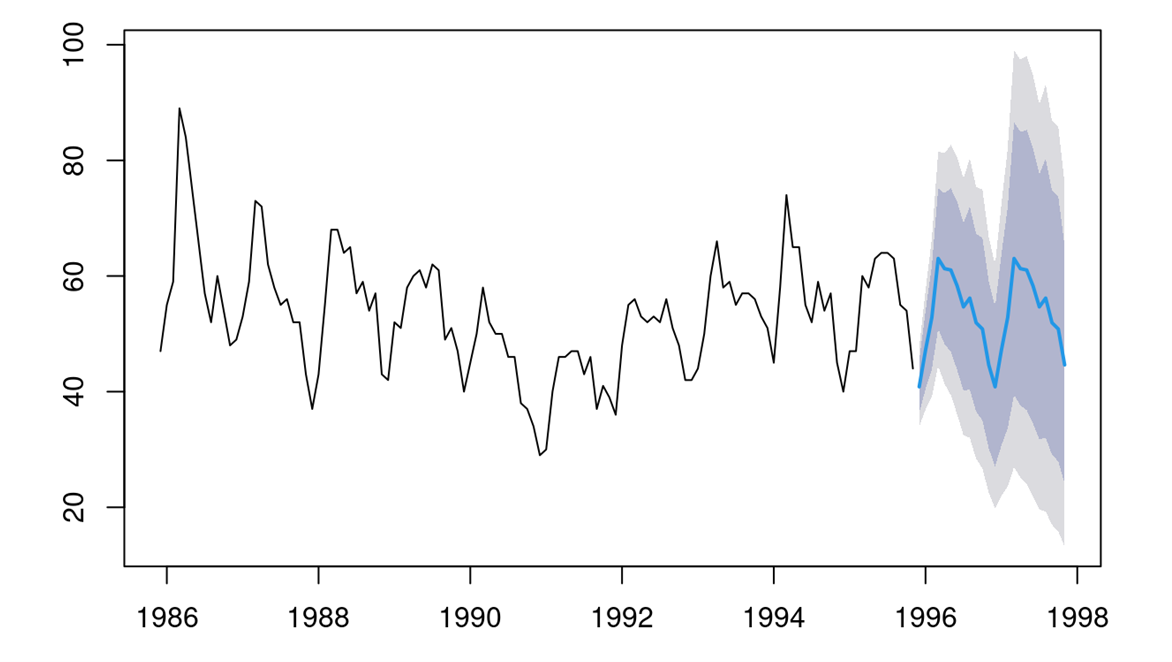
\includegraphics[width=10cm]{3_ChapterTranformerVariants/figuras/Probabilistic.png}
    \caption{Ilustration of Probabilistic Forecasting~\cite{hyndman2014visualization}}
    \LABFIG{FIG}
    \end{figure}





%%%%%%%%%%%%%%%%%%%%%%%%%%%%%%%%%%%%%%%%%%%%%%%%%%%%%%%%%%%%%%%%
\section{Informer}
In December 2020, Haoyi Zhou, Shanghang Zhang, Jieqi Peng, Shuai Zhang, Jianxin Li, Hui Xiong, and Wancai Zhang introduced a groundbreaking paper titled \textit{``Informer: Beyond Efficient Transformer for Long Sequence Time-Series Forecasting''}. This paper received the prestigious AAAI-21 Best Paper Award, recognizing its significant contributions to the field.

Next, we will delve into the core components of the Informer model. We will explore the ProbSparse Attention mechanism, which enhances efficiency and performance, and the Self-Attention Distilling technique, which optimizes the handling of long sequences. By understanding these innovations, we can appreciate how the Informer model significantly advances the capabilities of time-series forecasting.

\subsection{ProbSparse Attention}
The core concept of ProbSparse attention is based on the observation that canonical self-attention scores follow a long-tail distribution. In this distribution, ``active'' queries are located in the ``head'' scores, while ``lazy'' queries are found in the ``tail'' area. An ``active'' query, denoted as \( q_i \), is one where the dot-product \( \langle q_i, k_i \rangle \) significantly contributes to the attention mechanism. Conversely, a ``lazy'' query generates a dot-product that results in trivial attention. Here, \( q_i \) and \( k_i \) represent the \( i \)-th rows in the \( Q \) and \( K \) attention matrices, respectively.

Given the distinction between ``active'' and ``lazy'' queries, ProbSparse attention focuses on selecting the ``active'' queries to form a reduced query matrix \( Q_{\text{reduced}} \). This matrix is then used to compute the attention weights with a computational complexity of \( O(T \log T) \).

\begin{figure}[htbp]
    \centering
    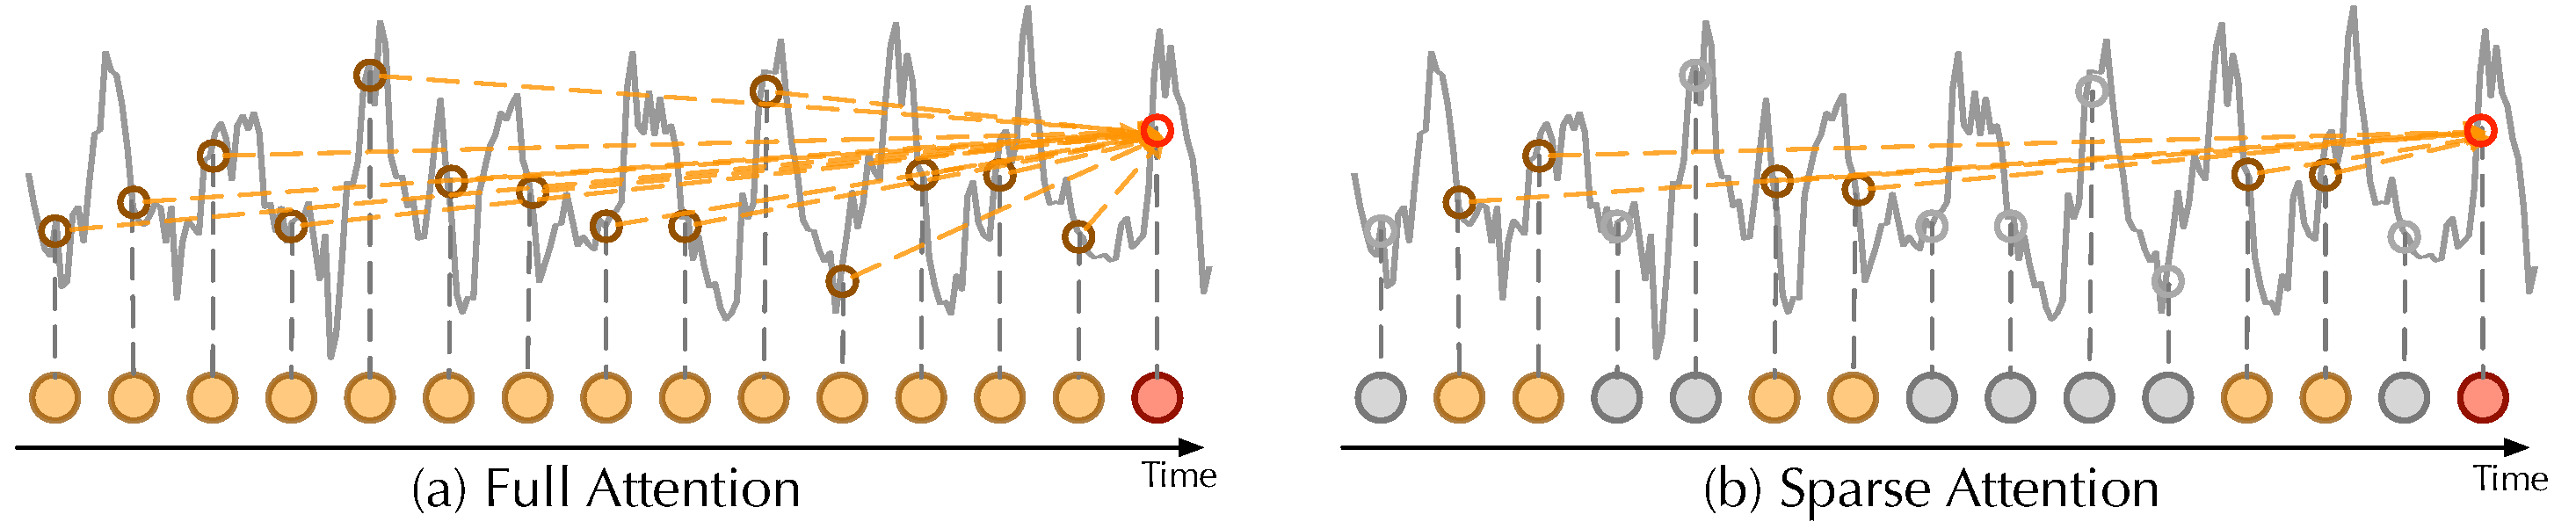
\includegraphics[width=15cm]{3_ChapterTranformerVariants/figuras/ProbSparceAttention.pdf}
    \caption{Vanilla self attention vs ProbSparse attention, from Autoformer (Wu, Haixu, et al., 2021)~\cite{wu2022autoformerdecompositiontransformersautocorrelation}}
    \LABFIG{FIG}
    \end{figure}

To illustrate this, let’s revisit the canonical self-attention formula:

\begin{equation}
\text{Attention}(Q, K, V) = \text{softmax}\left(\frac{QK^T}{\sqrt{d_k}}\right)V \text{ ,}
\end{equation}where \( Q \in \mathbb{R}^{L_Q \times d} \), \( K \in \mathbb{R}^{L_K \times d} \), and \( V \in \mathbb{R}^{L_V \times d} \). In practice, the input lengths of queries and keys are typically equivalent in self-attention computation, i.e., \( L_Q = L_K = T \), where \( T \) is the time series length. Consequently, the \( QK^T \) multiplication has a computational complexity of \( O(T^2 \cdot d) \).

In ProbSparse attention, the goal is to create a new \( Q_{\text{reduced}} \) matrix and define:

\begin{equation}
\text{ProbSparseAttention}(Q, K, V) = \text{softmax}\left(\frac{Q_{\text{reduced}} K^T}{\sqrt{d_k}}\right)V \text{ .}
\end{equation}

The \( Q_{\text{reduced}} \) matrix selects only the top \( u \) ``active'' queries, where \( u = c \cdot \log L_Q \) and \( c \) is the sampling factor hyperparameter for ProbSparse attention. Since \( Q_{\text{reduced}} \) selects only the top \( u \) queries, its size is \( c \cdot \log L_Q \times d \). Therefore, the multiplication \( Q_{\text{reduced}} K^T \) has a computational complexity of \( O(L_K \log L_Q) = O(T \log T) \).

The next step is to determine how to select the top \( u \) ``active'' queries to form \( Q_{\text{reduced}} \). This involves defining the Query Sparsity Measurement.
\vspace{10pt}

\noindent\textbf{Query Sparsity Measurement}

\vspace{10pt}
\noindent The Query Sparsity Measurement \( M(q_i, K) \) is used to identify the \( u \) ``active'' queries \( q_i \) within \( Q \) to construct \( Q_{\text{reduced}} \). The fundamental idea is that the dominant \( \langle q_i, k_i \rangle \) pairs cause the ``active'' \( q_i \)'s probability distribution to deviate from a uniform distribution. This deviation can be quantified using the KL divergence between the actual query distribution and the uniform distribution.

In practical terms, the measurement is defined as:

\begin{equation}
M(q_i, K) = \max_j \left( \frac{q_i k_j^T}{\sqrt{d}} \right) - \frac{1}{L_k} \sum_{j=1}^{L_k} \left( \frac{q_i k_j^T}{\sqrt{d}} \right) \text{ .}
\end{equation}

The key insight here is that a larger \( M(q_i, K) \) value indicates that the query \( q_i \) should be included in \( Q_{\text{reduced}} \), while a smaller value suggests otherwise.

To efficiently compute this measurement, it is important to note that most dot-products \( \langle q_i, k_i \rangle \) generate trivial attention due to the long-tail distribution property. Therefore, it is sufficient to consider a representative subset of keys from \( K \) rather than the entire set.

\begin{figure}[htbp]
    \centering
    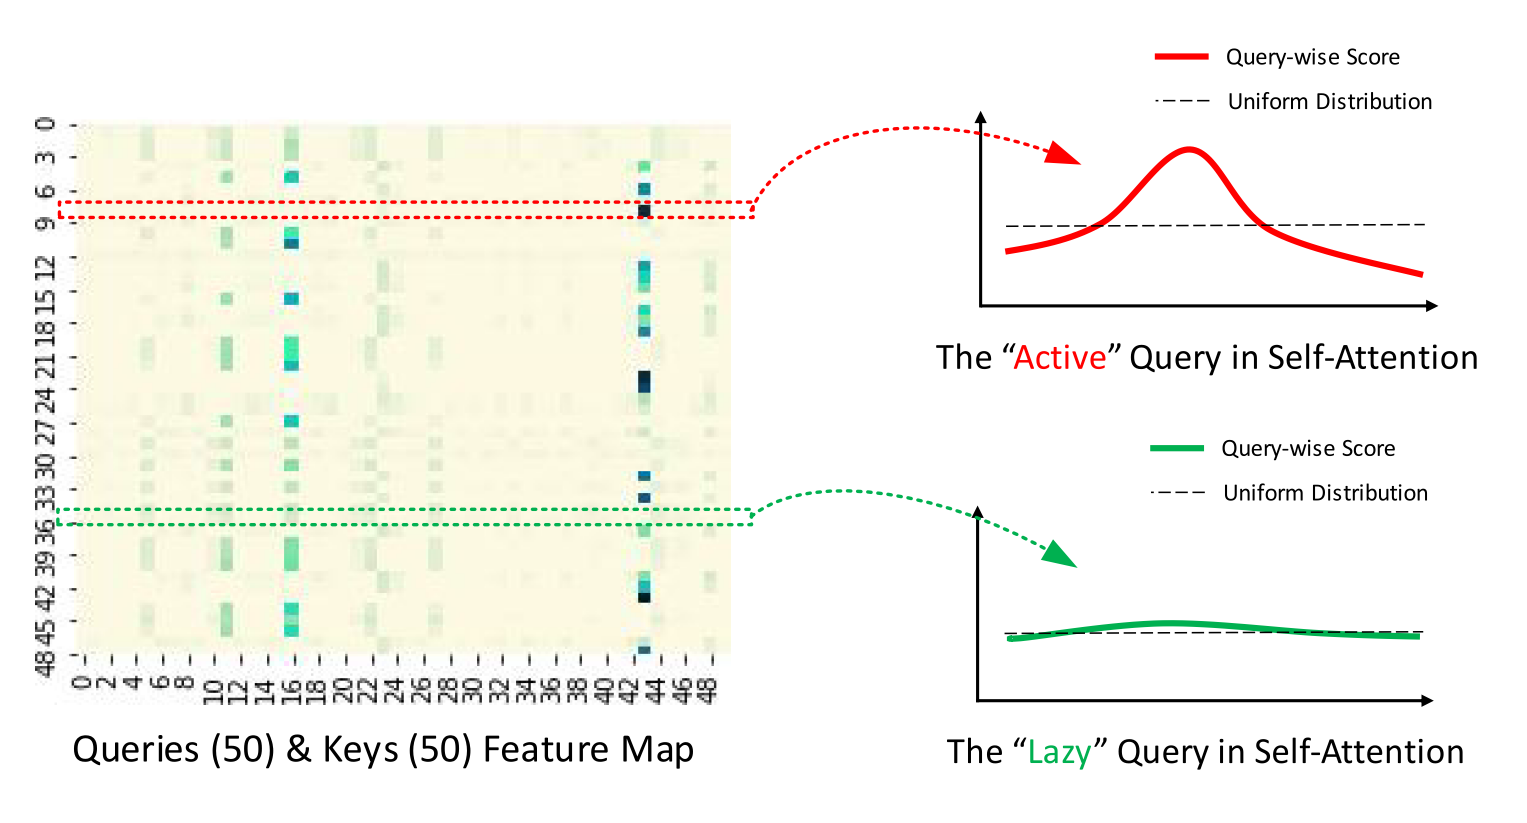
\includegraphics[width=12cm]{3_ChapterTranformerVariants/figuras/Queries_ProbSparceAttention.png}
    \caption{The illustration of ProbSparse Attention, from Informer (Zhou, et al., 2019)~\cite{zhou2021informerefficienttransformerlong}}
    \LABFIG{FIG}
    \end{figure}

\subsection{Distilling}
The Informer model employs a ProbSparse self-attention mechanism, which introduces some redundancy in the encoder’s feature map. To address this, a distilling operation is used to reduce the input size between encoder layers by half, effectively removing this redundancy. In practice, the distilling operation in Informer involves adding 1D convolution layers followed by max pooling between each of the encoder layers.

Let \( X_n \) be the output of the \( n \)-th encoder layer. The distilling operation is then defined as:

\begin{equation}
X_{n+1} = \text{MaxPool}(\text{ELU}(\text{Conv1d}(X_n)))
\end{equation}

By applying this operation, the input size of each subsequent layer is reduced by half. This reduction leads to a more efficient memory usage. Specifically, the memory usage is reduced from \( O(N \cdot T^2) \) to \( O(N \cdot T \log T) \), where \( N \) is the number of encoder/decoder layers and \( T \) is the sequence length. This optimization is crucial for handling long sequence time-series forecasting tasks efficiently.



%%%%%%%%%%%%%%%%%%%%%%%%%%%%%%%%%%%%%%%%%%%%%%%%%%%%%%%%%%%%%%%%
\section{Autoformer}
In June 2021, Haixu Wu, Jiehui Xu, Jianmin Wang, and Mingsheng Long introduced an innovative paper titled \textit{``Autoformer: Decomposition Transformers with Auto-Correlation for Long-Term Series Forecasting’'}. This paper has been widely recognized for its significant contributions to the field of long-term time series forecasting.

Autoformer enhances the transformer architecture by incorporating time series decomposition and a unique auto-correlation mechanism. In the following, we will explain the main contributions of Autoformer, focusing on the Decomposition Layer and the Attention (Autocorrelation) Mechanism. These innovations allow Autoformer to capture and leverage period-based dependencies, enhancing its performance over traditional transformer models.

\subsection{Decomposition Layer}

Time series decomposition is a method of breaking down a time series into three systematic components: trend-cycle, seasonal variation, and random fluctuations. The trend component reflects the long-term direction of the series, which can be increasing, decreasing, or stable. The seasonal component captures recurring patterns within the series, such as yearly or quarterly cycles. The random component represents the noise that cannot be explained by the trend or seasonal components.

Decomposition can be either additive, where the components are summed, or multiplicative, where the components are multiplied. This technique, commonly implemented in libraries like \textit{statsmodels}, helps in understanding and modeling the underlying patterns in the data.

\subsubsection{Decomposition in Autoformer}
Autoformer incorporates a decomposition block within its architecture. This block enables the model to progressively aggregate the trend-cyclical part and extract the seasonal part from the series. The encoder and decoder of Autoformer use this decomposition block, significantly enhancing the model’s ability to capture and utilize these components.

Formally, for an input series \( X \in \mathbb{R}^{L \times d} \) with length \( L \), the decomposition layer returns \( X_{\text{trend}} \) and \( X_{\text{seasonal}} \) defined as:

\begin{equation}
X_{\text{trend}} = \text{AvgPool}(\text{Padding}(X)) \text{ ,}
\end{equation}

\begin{equation}
X_{\text{seasonal}} = X - X_{\text{trend}} \text{ .}
\end{equation}

This decomposition layer allows Autoformer to explicitly model the trend and seasonal components, which has proven beneficial in various time series forecasting applications.

\begin{figure}[htbp]
    \centering
    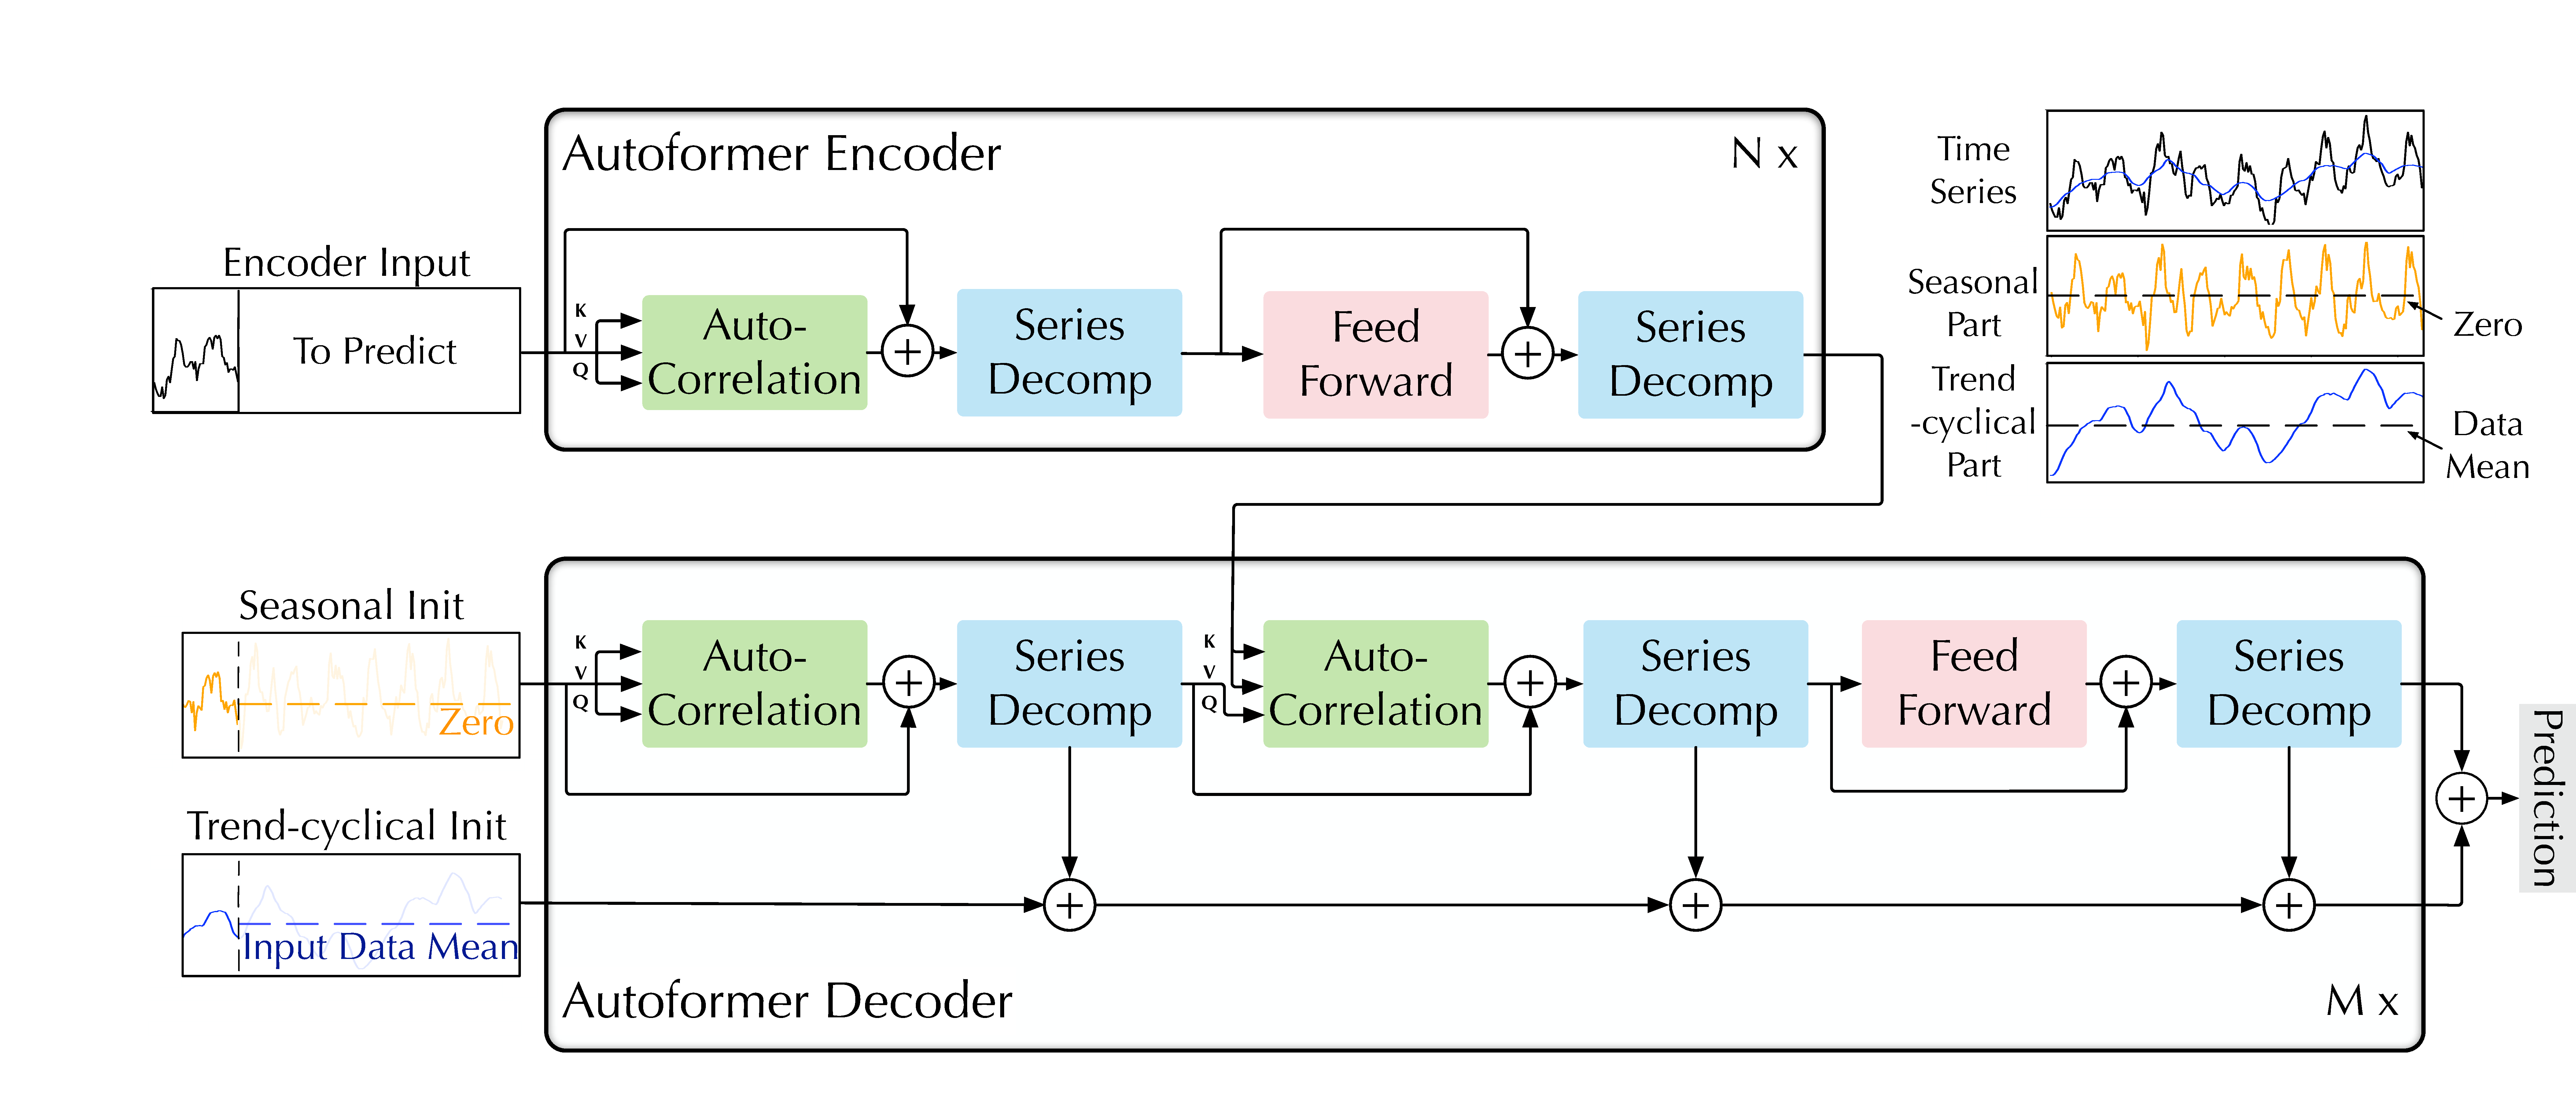
\includegraphics[width=15cm]{3_ChapterTranformerVariants/figuras/AutoformerArchitecture.pdf}
    \caption{Autoformer architecture. The encoder eliminates the long-term trend-cyclical part by series decomposition blocks (\textcolor{blue}{blue} blocks) and focuses on seasonal patterns modeling. The decoder accumulates the trend part extracted from hidden variables progressively. The past seasonal information from encoder is utilized by the encoder-decoder Auto-Correlation (center \textcolor[rgb]{0.15,0.7,0.15}{green} block in decoder), from Autoformer (Wu, Haixu, et al., 2021)~\cite{wu2022autoformerdecompositiontransformersautocorrelation}}
    \LABFIG{FIG}
    \end{figure}



\subsection{Attention (Autocorrelation) Mechanism}
Autoformer introduces an innovative approach to the attention mechanism used in traditional transformers. Instead of the conventional self-attention, which calculates attention weights directly in the time domain, Autoformer utilizes an autocorrelation mechanism that operates in the frequency domain using the Fast Fourier Transform (FFT). This method helps the model better capture periodic dependencies in the data, thereby enhancing its forecasting performance.

\subsubsection{Understanding Autocorrelation}
Autocorrelation, also known as serial correlation, measures how a time series correlates with a lagged version of itself over successive time intervals. It is a crucial concept in time series analysis, as it helps identify patterns, trends, and periodic fluctuations within the data.

For a given time lag \( \tau \), autocorrelation quantifies the relationship (often measured by Pearson correlation) between the current value of the series at time \( t \) and its past value at time \( t - \tau \). Mathematically, it is expressed as:

\begin{equation}
\text{Autocorrelation}(\tau) = \text{Corr}(y_t, y_{t-\tau}) \text{ ,}
\end{equation}where \( y_t \) represents the value of the time series at time \( t \), and \( y_{t-\tau} \) represents the value at time \( t - \tau \).

Autocorrelation values range from -1 to 1:
\begin{itemize}
    \item A value of 1 indicates perfect positive correlation, meaning the series is perfectly aligned with its past values.
    \item A value of -1 indicates perfect negative correlation, meaning the series is perfectly inversely aligned with its past values.
    \item A value of 0 indicates no correlation, meaning there is no linear relationship between the current and past values.
\end{itemize}

In the context of Autoformer, this concept replaces the traditional dot-product attention mechanism used in transformers. Instead of directly comparing queries (Q) and keys (K) through dot-products, Autoformer leverages autocorrelation to capture dependencies over different time lags. This approach allows Autoformer to effectively model long-term dependencies and seasonal patterns in time series data, leading to improved forecasting performance.

\begin{figure}[htbp]
    \centering
    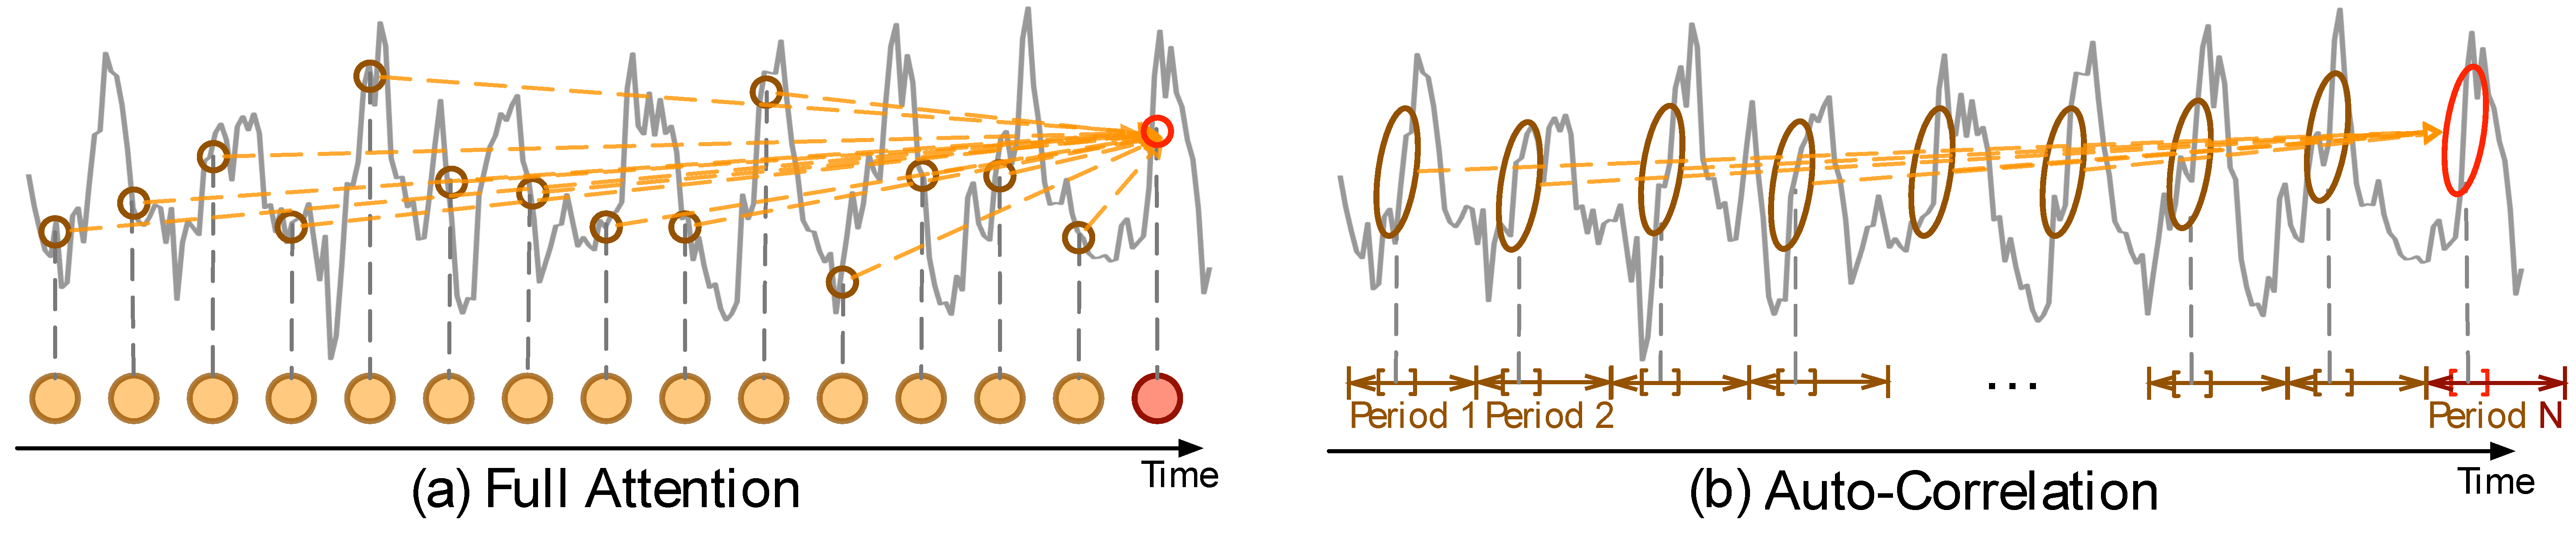
\includegraphics[width=15cm]{3_ChapterTranformerVariants/figuras/FullAttentionAutoCorrelation.pdf}
    \caption{Vanilla self attention vs Autocorrelation mechanism, from Autoformer (Wu, Haixu, et al., 2021)~\cite{wu2022autoformerdecompositiontransformersautocorrelation}}
    \LABFIG{FIG}
    \end{figure}


\subsubsection{Implementing Autocorrelation with FFT}
The autocorrelation mechanism computes the attention weights using the Fast Fourier Transform (FFT). The FFT is an efficient algorithm to compute the Discrete Fourier Transform (DFT) and its inverse. It transforms a sequence of complex numbers into another sequence, representing the original sequence in the frequency domain. This approach allows all lags’ autocorrelations to be calculated simultaneously, making the process efficient with a time complexity of \( O(L \log L) \), where \( L \) is the length of the input time series.

Here’s how it works in practice:
\begin{enumerate}
    \item \textbf{FFT Transformation:} Convert the queries (Q) and keys (K) from the time domain to the frequency domain using FFT. This involves decomposing the input sequences into a sum of sinusoids of different frequencies, which represent the original data in the frequency domain.
    \item \textbf{Frequency Domain Multiplication:} Multiply the transformed Q and K element-wise in the frequency domain. This step leverages the convolution theorem, which states that convolution in the time domain corresponds to point-wise multiplication in the frequency domain.
    \item \textbf{Inverse FFT:} Apply the inverse FFT to transform the results back from the frequency domain to the time domain. This step reconstructs the autocorrelations from the frequency domain representation, yielding the desired autocorrelation values.
\end{enumerate}
    

\begin{figure}[htbp]
    \centering
    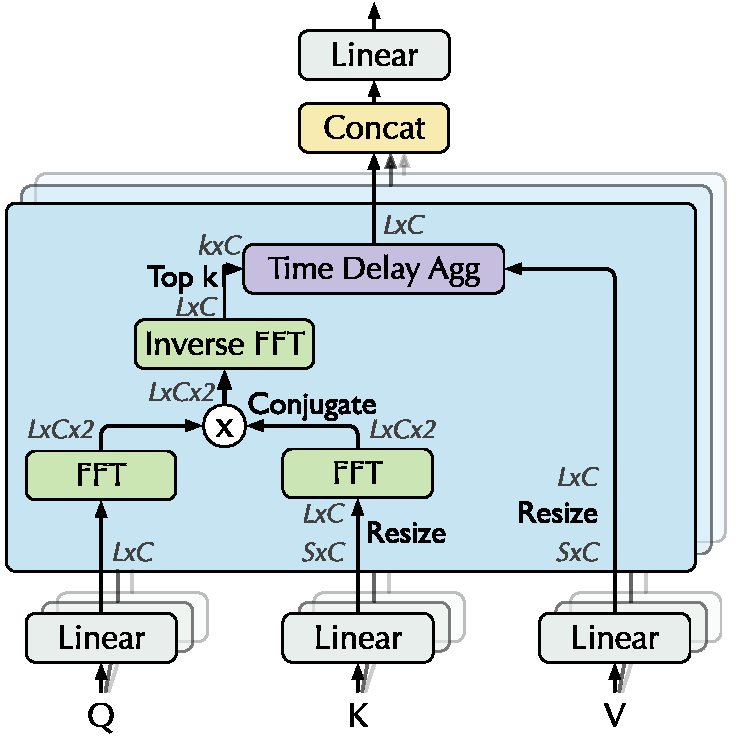
\includegraphics[width=8cm]{3_ChapterTranformerVariants/figuras/AttentionWeightsComputation.pdf}
    \caption{Attention weights computation in frequency domain using FFT, from Autoformer (Wu, Haixu, et al., 2021)~\cite{wu2022autoformerdecompositiontransformersautocorrelation}}
    \LABFIG{FIG}
    \end{figure}



\subsubsection{Time Delay Aggregation}
Time Delay Aggregation (TDA) is a crucial step in the Autoformer model, designed to effectively capture the periodic dependencies in time series data. By aggregating information over different time delays, TDA ensures that the model can efficiently utilize the data, leading to better forecasting performance and improved accuracy for long-term time series forecasting.

Once the autocorrelation weights (referred to as \textit{attn\_weights}) are computed, they need to be aggregated with the values (V) to produce the final attention output. This process involves the following steps:

\begin{enumerate}
    \item \textbf{Rolling:} For each time delay \( \tau \), align the values (V) by shifting them by \( \tau \). This process is called rolling. It helps in aligning the values with their corresponding time delays, ensuring that the periodic patterns are captured accurately.
    \item \textbf{Element-wise Multiplication:} Multiply the rolled values by the corresponding autocorrelation weights. This step ensures that the influence of each time delay is weighted according to its importance, as determined by the autocorrelation weights.
    \item \textbf{Summation:} Sum the weighted values to get the final attention output. This aggregation step combines the information from different time delays, providing a comprehensive representation of the periodic dependencies in the data.
\end{enumerate}

The aggregation process can be formalized with the following equations:

\begin{enumerate}
    \item Identify the top-k lags with the highest autocorrelation values:
    \begin{equation}
    \tau_1, \tau_2, \ldots, \tau_k = \text{arg Top-k}(R_{Q,K}(\tau))
    \end{equation}
    \item Apply softmax to normalize the autocorrelation values:
    \begin{equation}
    \hat{R}_{Q,K}(\tau_1), \hat{R}_{Q,K}(\tau_2), \ldots, \hat{R}_{Q,K}(\tau_k) = \text{Softmax}(R_{Q,K}(\tau_1), R_{Q,K}(\tau_2), \ldots, R_{Q,K}(\tau_k))
    \end{equation}
    \item Compute the final attention output by summing the element-wise products of the rolled values and the normalized autocorrelation weights:
    \begin{equation}
    \text{Autocorrelation-Attention} = \sum_{i=1}^{k} \text{Roll}(V, \tau_i) \cdot \hat{R}_{Q,K}(\tau_i)
    \end{equation}
\end{enumerate}

\begin{figure}[htbp]
    \centering
    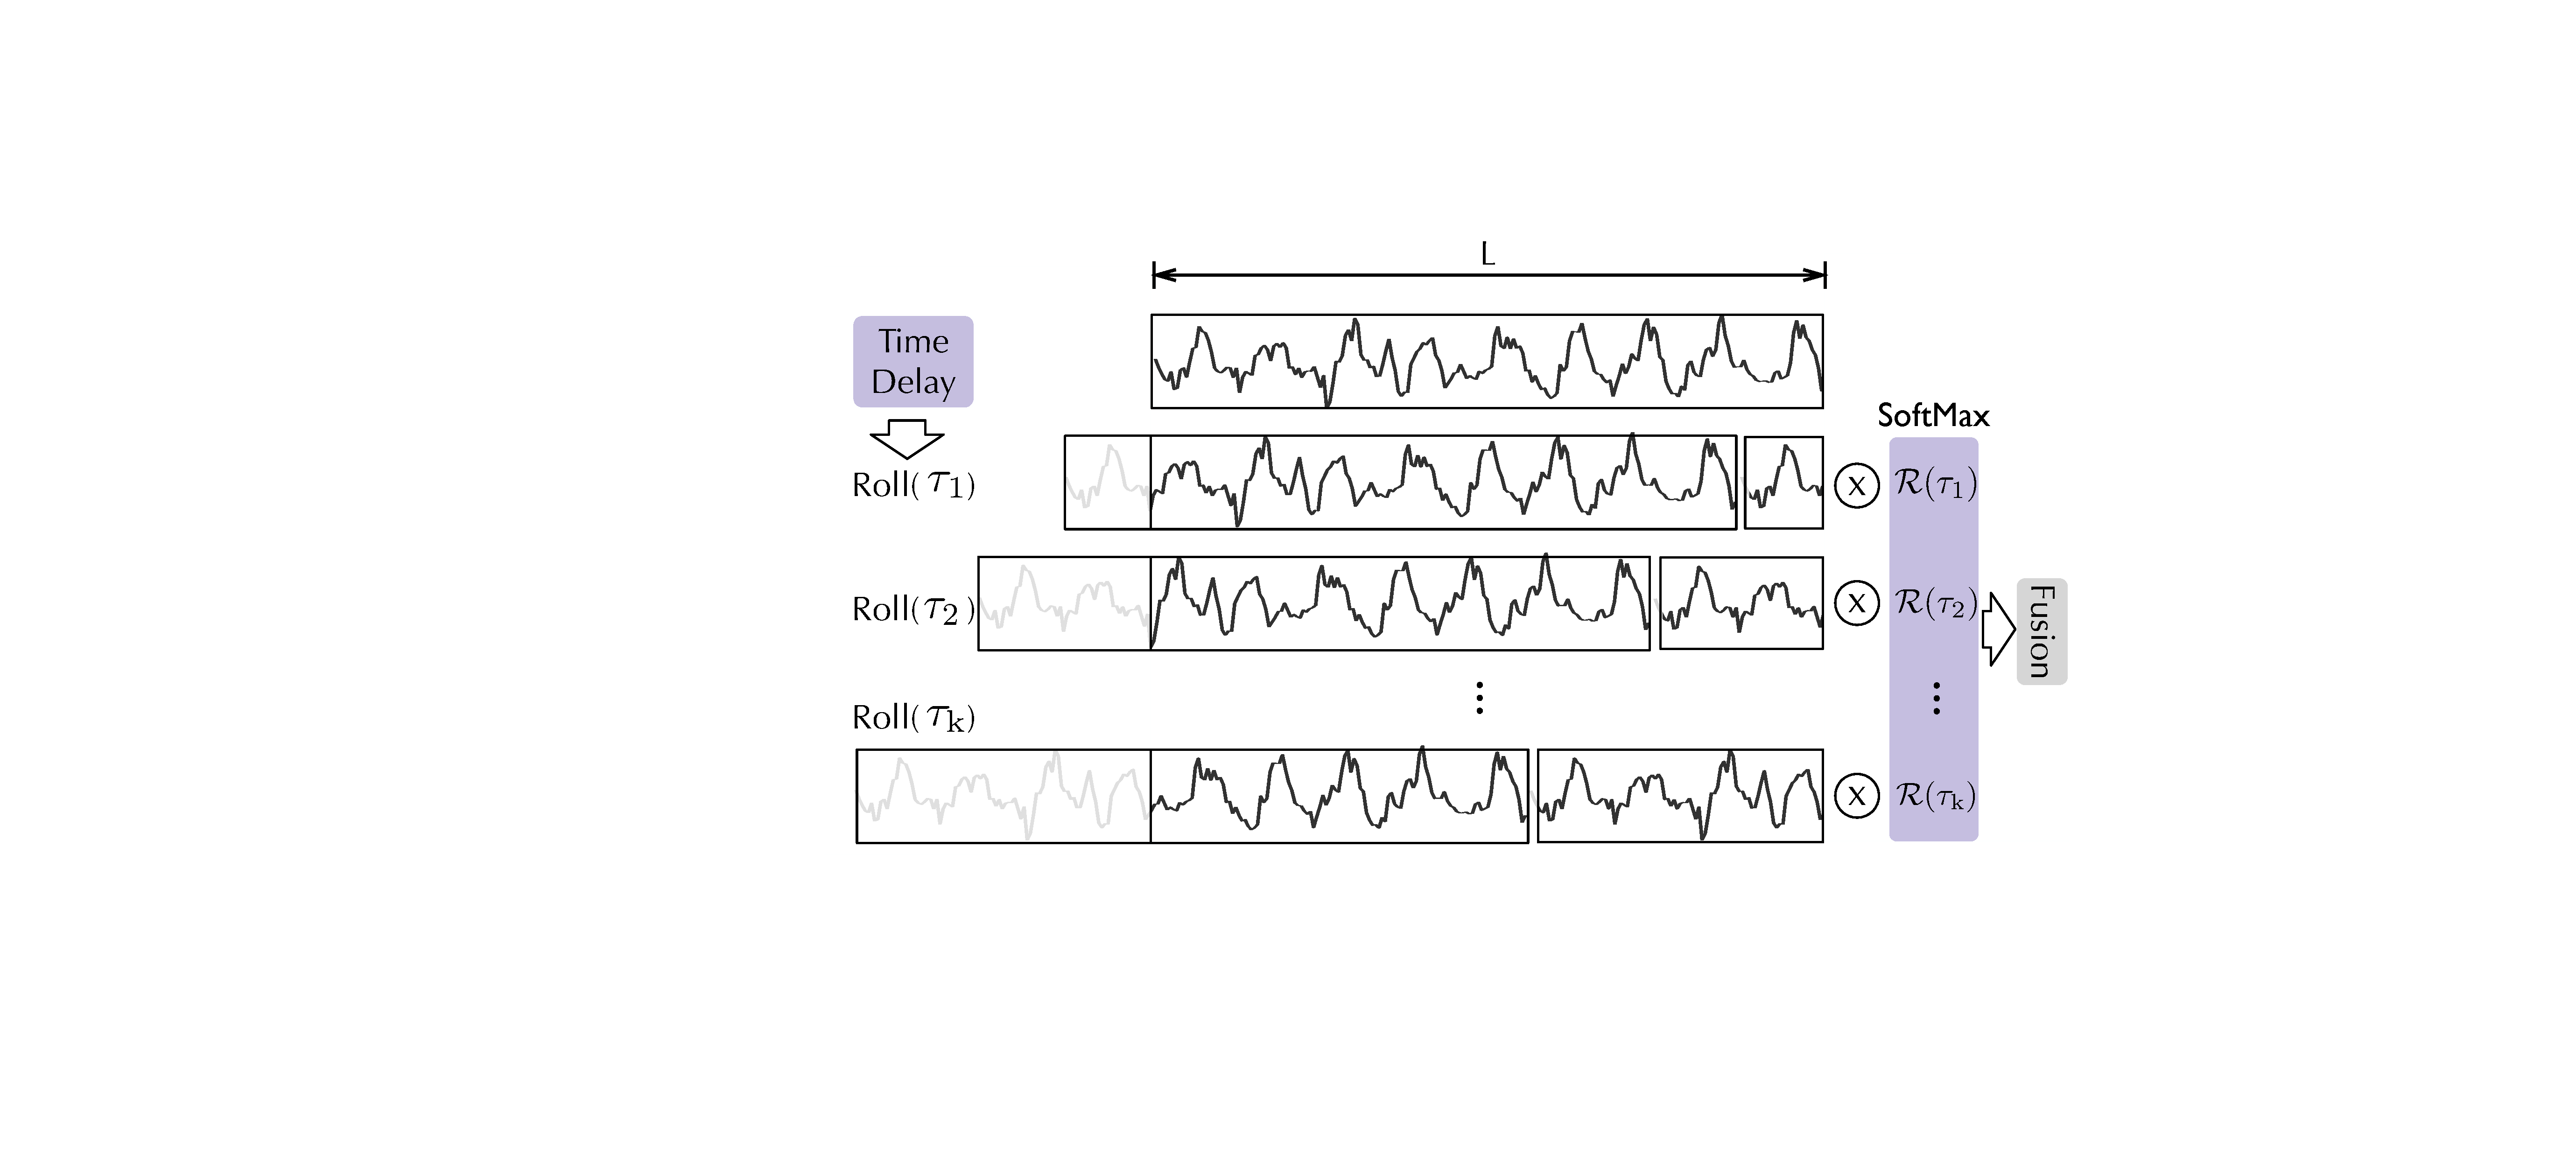
\includegraphics[width=12cm]{3_ChapterTranformerVariants/figuras/TimeDelay.pdf}
    \caption{Aggregation by time delay, from Autoformer (Wu, Haixu, et al., 2021)~\cite{wu2022autoformerdecompositiontransformersautocorrelation}}
    \LABFIG{FIG}
    \end{figure}

